% Template for PLoS
% Version 3.6 Aug 2022
%
% % % % % % % % % % % % % % % % % % % % % %
%
% -- IMPORTANT NOTE
%
% This template contains comments intended 
% to minimize problems and delays during our production 
% process. Please follow the template instructions
% whenever possible.
%
% % % % % % % % % % % % % % % % % % % % % % % 
%
% Once your paper is accepted for publication, 
% PLEASE REMOVE ALL TRACKED CHANGES in this file 
% and leave only the final text of your manuscript. 
% PLOS recommends the use of latexdiff to track changes during review, as this will help to maintain a clean tex file.
% Visit https://www.ctan.org/pkg/latexdiff?lang=en for info or contact us at latex@plos.org.
%
%
% There are no restrictions on package use within the LaTeX files except that no packages listed in the template may be deleted.
%
% Please do not include colors or graphics in the text.
%
% The manuscript LaTeX source should be contained within a single file (do not use \input, \externaldocument, or similar commands).
%
% % % % % % % % % % % % % % % % % % % % % % %
%
% -- FIGURES AND TABLES
%
% Please include tables/figure captions directly after the paragraph where they are first cited in the text.
%
% DO NOT INCLUDE GRAPHICS IN YOUR MANUSCRIPT
% - Figures should be uploaded separately from your manuscript file. 
% - Figures generated using LaTeX should be extracted and removed from the PDF before submission. 
% - Figures containing multiple panels/subfigures must be combined into one image file before submission.
% For figure citations, please use "Fig" instead of "Figure".
% See http://journals.plos.org/plosone/s/figures for PLOS figure guidelines.
%
% Tables should be cell-based and may not contain:
% - spacing/line breaks within cells to alter layout or alignment
% - do not nest tabular environments (no tabular environments within tabular environments)
% - no graphics or colored text (cell background color/shading OK)
% See http://journals.plos.org/plosone/s/tables for table guidelines.
%
% For tables that exceed the width of the text column, use the adjustwidth environment as illustrated in the example table in text below.
%
% % % % % % % % % % % % % % % % % % % % % % % %
%
% -- EQUATIONS, MATH SYMBOLS, SUBSCRIPTS, AND SUPERSCRIPTS
%
% IMPORTANT
% Below are a few tips to help format your equations and other special characters according to our specifications. For more tips to help reduce the possibility of formatting errors during conversion, please see our LaTeX guidelines at http://journals.plos.org/plosone/s/latex
%
% For inline equations, please be sure to include all portions of an equation in the math environment.  For example, x$^2$ is incorrect; this should be formatted as $x^2$ (or $\mathrm{x}^2$ if the romanized font is desired).
%
% Do not include text that is not math in the math environment. For example, CO2 should be written as CO\textsubscript{2} instead of CO$_2$.
%
% Please add line breaks to long display equations when possible in order to fit size of the column. 
%
% For inline equations, please do not include punctuation (commas, etc) within the math environment unless this is part of the equation.
%
% When adding superscript or subscripts outside of brackets/braces, please group using {}.  For example, change "[U(D,E,\gamma)]^2" to "{[U(D,E,\gamma)]}^2". 
%
% Do not use \cal for caligraphic font.  Instead, use \mathcal{}
%
% % % % % % % % % % % % % % % % % % % % % % % % 
%
% Please contact latex@plos.org with any questions.
%
% % % % % % % % % % % % % % % % % % % % % % % %

\documentclass[10pt,letterpaper]{article}
\usepackage[top=0.85in,left=2.75in,footskip=0.75in]{geometry}

% amsmath and amssymb packages, useful for mathematical formulas and symbols
\usepackage{amsmath,amssymb}

% Use adjustwidth environment to exceed column width (see example table in text)
\usepackage{changepage}

% textcomp package and marvosym package for additional characters
\usepackage{textcomp,marvosym}

% cite package, to clean up citations in the main text. Do not remove.
\usepackage{cite}

% Use nameref to cite supporting information files (see Supporting Information section for more info)
\usepackage{nameref,hyperref}

% line numbers
\usepackage[right]{lineno}

% ligatures disabled
\usepackage[nopatch=eqnum]{microtype}
\DisableLigatures[f]{encoding = *, family = * }

% color can be used to apply background shading to table cells only
%\usepackage[table]{xcolor}

% array package and thick rules for tables
\usepackage{array}

% create "+" rule type for thick vertical lines
\newcolumntype{+}{!{\vrule width 2pt}}

% create \thickcline for thick horizontal lines of variable length
\newlength\savedwidth
\newcommand\thickcline[1]{%
  \noalign{\global\savedwidth\arrayrulewidth\global\arrayrulewidth 2pt}%
  \cline{#1}%
  \noalign{\vskip\arrayrulewidth}%
  \noalign{\global\arrayrulewidth\savedwidth}%
}

% \thickhline command for thick horizontal lines that span the table
\newcommand\thickhline{\noalign{\global\savedwidth\arrayrulewidth\global\arrayrulewidth 2pt}%
\hline
\noalign{\global\arrayrulewidth\savedwidth}}


% Remove comment for double spacing
%\usepackage{setspace} 
%\doublespacing

% Text layout
\raggedright
\setlength{\parindent}{0.5cm}
\textwidth 5.25in 
\textheight 8.75in

% Bold the 'Figure #' in the caption and separate it from the title/caption with a period
% Captions will be left justified
\usepackage[aboveskip=1pt,labelfont=bf,labelsep=period,justification=raggedright,singlelinecheck=off]{caption}
\renewcommand{\figurename}{Fig}

% Use the PLoS provided BiBTeX style
\bibliographystyle{plos2015}

% Remove brackets from numbering in List of References
\makeatletter
\renewcommand{\@biblabel}[1]{\quad#1.}
\makeatother



% Header and Footer with logo
\usepackage{lastpage,fancyhdr,graphicx}
\usepackage{epstopdf}
\usepackage{lmodern}
%\pagestyle{myheadings}
\pagestyle{fancy}
\fancyhf{}
%\setlength{\headheight}{27.023pt}
%\lhead{\includegraphics[width=2.0in]{PLOS-submission.eps}}
\rfoot{\thepage/\pageref{LastPage}}
\renewcommand{\headrulewidth}{0pt}
\renewcommand{\footrule}{\hrule height 2pt \vspace{2mm}}
\fancyheadoffset[L]{2.25in}
\fancyfootoffset[L]{2.25in}
\lfoot{\today}

%% Include all macros below

\newcommand{\lorem}{{\bf LOREM}}
\newcommand{\ipsum}{{\bf IPSUM}}

%% END MACROS SECTION

%% personal packages and macro
%%% packages
\usepackage[utf8]{inputenc}        % allow utf-8 input
\usepackage[T1]{fontenc}           % use 8-bit T1 fonts
\usepackage[dvipsnames, table]{xcolor}
\usepackage{tabularx}
\usepackage{multirow}
\usepackage{pifont}
\usepackage{csvsimple}
\usepackage[font={small},textfont={it},labelfont={bf}]{caption}
\usepackage{subcaption}
\usepackage{graphicx}
\usepackage{url}                   % simple URL typesetting
\usepackage{booktabs}              % professional-quality tables
\usepackage{makecell}
\usepackage{amsfonts}              % blackboard math symbols
\usepackage{amsmath}
\usepackage{nicefrac}              % compact symbols for 1/2, etc.
\usepackage{microtype}             % microtypography
\usepackage{enumitem}
\usepackage[export]{adjustbox}


%not compatible with cite package
%\usepackage[natbib=true,style=nature,maxnames=999,maxcitenames=2,backend=biber]{biblatex}
%\addbibresource{references.bib}

%%% macros
\DeclareMathOperator*{\argmin}{arg\,min}
\newcommand{\indep}{\perp \!\!\! \perp}
\newtheorem{assumption}{Assumption}

\definecolor{dark_blue}{rgb}{0,0,.65}
\definecolor{dark_green}{rgb}{0,.5,.15}

\hypersetup{pdftex,  % needed for pdflatex
  breaklinks=true,  % so long urls are correctly broken across lines
  colorlinks=true,
  linkcolor=dark_blue,
  citecolor=dark_green,
}
\colorlet{P}{ForestGreen}
\colorlet{I}{MidnightBlue}
\colorlet{C}{YellowOrange}
\colorlet{O}{DarkOrchid}
\colorlet{T}{Gray}



\begin{document}
\vspace*{0.2in}

% Title must be 250 characters or less.
\begin{flushleft}
  {\Large
    \textbf\newline{Step-by-step causal analysis of EHRs to ground decision-making} % Please use "sentence case" for title and headings (capitalize only the first word in a title (or heading), the first word in a subtitle (or subheading), and any proper nouns).
  }
  \newline
  % Insert author names, affiliations and corresponding author email (do not include titles, positions, or degrees).
  \\
  Matthieu Doutreligne\textsuperscript{1,2,*},
  Tristan Struja\textsuperscript{3,4},
  Judith Abecassis\textsuperscript{1},
  Claire Morgand\textsuperscript{5},
  Leo Anthony Celi\textsuperscript{3,6,7},
  Gaël Varoquaux\textsuperscript{1}
  \bigskip
  \textbf{1} Inria, Soda, Saclay, France
  \\
  \textbf{2} Mission Data, Haute Autorité de Santé, Saint-Denis, France
  \\
  \textbf{3} Laboratory for Computational Physiology, Massachusetts Institute of Technology, Cambridge, MA 02139
  \\
  \textbf{4} Medical University Clinic, Division of Endocrinology, Diabetes \& Metabolism, Kantonsspital Aarau, Aarau, Switzerland
  \\
  \textbf{5} Agence Régionale de Santé Ile-de-France, France
  \\
  \textbf{6} Division of Pulmonary, Critical Care and Sleep Medicine, Beth Israel Deaconess Medical Center, Boston, MA 02215
  \\
  \textbf{7} Department of Biostatistics, Harvard T.H. Chan School of Public Health, Boston, MA 02115
  \bigskip




  % Insert additional author notes using the symbols described below. Insert symbol callouts after author names as necessary.
  % 
  % Remove or comment out the author notes below if they aren't used.
  %
  % Primary Equal Contribution Note
  %\Yinyang Corresponding author: m.doutreligne@has-sante.fr.

  % Additional Equal Contribution Note
  % Also use this double-dagger symbol for special authorship notes, such as senior authorship.
  %\ddag These authors also contributed equally to this work.

  % Current address notes
  %\textcurrency Current Address: Dept/Program/Center, Institution Name, City, State, Country % change symbol to "\textcurrency a" if more than one current address note
  % \textcurrency b Insert second current address 
  % \textcurrency c Insert third current address

  % Deceased author note
  %\dag Deceased

  % Group/Consortium Author Note
  %\textpilcrow Membership list can be found in the Acknowledgments section.

  % Use the asterisk to denote corresponding authorship and provide email address in note below.
  * Corresponding author: m.doutreligne@has-sante.fr


\end{flushleft}
% Please keep the abstract below 300 words --> 235
\section*{Abstract}

Causal inference enables machine learning methods to estimate
treatment effects of medical interventions from electronic health
records (EHRs). However, researchers should be wary of many pitfalls.
Here we explain and study common pitfalls and potential solutions,
estimating the effect of albumin on mortality in sepsis using an
Intensive Care database (MIMIC-IV) and comparing to outcome data from randomized
controlled trials (RCT) as gold-standard. The first step is study design,
using the target trial concept and the PICOT framework: Population
(patients with sepsis), Intervention (combination of crystalloids and albumin
for fluid resuscitation), Control (crystalloids only), Outcome (28-day
mortality), Time (intervention start within 24h of admission).
We show that a too large treatment-initiation time induces immortal time bias.
The second step is
selection of the confounding variables based on expert knowledge.
Increasingly adding confounders enables to recover the RCT results from
observational data (0\%, 95\% CI -1\% to 1\%, and 0\%, 95\% -5\% to 5\%,
respectively).
The third step is fitting outcome models, and we assess the influence of
multiple models with varying assumptions. A doubly
robust estimator (AIPW) with random forests proved to be the most reliable
estimator. Results show that these steps are all important for valid
causal estimates. A valid causal model can then be used to individualize
decision making:
subgroup analyses showed that treatment efficacy of albumin was better for
patients >60 years old, males, and patients with septic shock.

% Please keep the Author Summary between 150 and 200 words
% Use first person. PLOS ONE authors please skip this step. 
% Author Summary not valid for PLOS ONE submissions.   
\section*{Author summary}

Rich routine-care data, as EHR or claims, is useful to individualize decision
making using machine learning; but guiding interventions requires
causal inference. Unlike with an RCT, interventions in routine data do
not easily enable an apple-to-apple measure of the effect of an
intervention, leading to many analytical pitfalls, particularly in
time-varying data. We study these in a tutorial spirit, making
the code and data openly available. We give 5 analytical steps for
data-driven individualized interventions: Step
1) Study design, where common pitfalls are selection bias, with information
unequally collected across treatment and control patients, and immortal time
bias, where the inclusion-defining event interacts with the
intervention time. Step 2) Identification of the causal assumptions and
categorization of confounders. Step 3) Estimation of the causal effect of
interest by correct aggregation of confounders and selection of an appropriate
statistical model. Step 4) Assessing the
analysis' robustness to assumptions, and finally Step 5) Individualizing
treatment decision, by exploring treatment heterogeneity, eg across subgroups.
Studying choice of fluid resuscitation in sepsis, we show that common
mistakes in steps 1, 2, and 3 equally compromise causal validity.


\linenumbers

% Use "Eq" instead of "Equation" for equation citations.
\section*{Introduction: data-driven decisions require causal inference}
%\label{introduction}

Informing a care option extends beyond merely predicting the occurrence
of an event; it involves estimating the effect of the corresponding
treatment effects. Routine-care data comes naturally to mind to guide
routine decisions, but they require care to estimate treatment effects as
they are observational, unlike Randomized controlled trials (RCTs). This
context calls for causal inference statistical frameworks.
But merely applying these tools to the data does suffice to ensure the
validity of the inferences; numerous considerations must be carefully addressed.

\paragraph{Individualized Medicine and Machine Learning Challenges}
Machine learning plays a pivotal role in individualized medicine  \cite{rajkomar2018scalable,liu2019comparison,li2020behrt,beaulieu2021machine,aggarwal2021diagnostic}. It
demonstrated superior performance over traditional rule-based clinical scores in predicting a patient's readmission risk, mortality, or future comorbidities using Electronic Health Records (EHRs) \cite{rajkomar2018scalable,liu2019comparison,li2020behrt,beaulieu2021machine,aggarwal2021diagnostic}.
However, mounting evidence suggests that machine-learning models can inadvertently perpetuate and exacerbate biases present in the data \cite{rajkomar2018ensuring}, including gender or racial biases \cite{singh2022generalizability,gichoya2022ai}, and the marginalization of under-served populations \cite{seyyed2021underdiagnosis}. These biases are typically encoded by capturing shortcuts—stereotypical or distorted features in the data \cite{geirhos2020shortcut,winkler2019association,degrave2021ai}.
%
For instance, numerous machine learning algorithms rely on post-treatment information \cite{badgeley2019deep,obermeyer2019dissecting,yuan2021temporal,wong2021external}, exemplified by a diagnostic model for skin cancer that depends on surgical marks \cite{winkler2019association}. For Intensive Care Unit data, focus of our study, such information markedly improves mortality prediction (Figure S1 \ref{apd:fig:motivating_example}), but cannot inform decisions.

\paragraph{The Importance of Causal Reasoning in Data-Driven Decision-Making} \cite{prosperi2020causal}
While conventional machine learning relies on retrospective to generate predictions of future effects \cite{plecko2022causal}, truly informing decision-making needs a comparison of potential outcomes with and without the intervention. This involves estimating a causal effect, mirroring the methodology employed in RCTs \cite{prosperi2020causal}. However, RCTs encounter challenges such as selection biases \cite{travers2007external,averitt2020translating}, difficulties in recruiting diverse populations, and limited sample sizes for exploring treatment heterogeneity across subgroups. Routinely collected data presents a unique opportunity to assess real-life benefit-risk trade-offs associated with a decision \cite{desai2021broadening}, with reduced sampling bias and sufficient data to capture heterogeneity \cite{rekkas2023standardized}. Nevertheless, estimating causal effects from such data is challenging due to the confounding of the intervention by indication. Therefore, dedicated statistical techniques are imperative to emulate a "target trial" \cite{hernan2016specifying} from observational data.

\paragraph{How lack of individual treatment model limits a cardiovascular risk score}
The QRISK is a risk score widely used in the UK to assess 10-year and lifetime cardio-vascular risk \cite{hippisley2017development}. It is well calibrated, recommended by the national regulatory agency \cite{guideline2023cardiovascular}, and the National Institute for Health and Care Excellence (NICE) argues to use such a score to systematically screen cardio-vascular disease (CVD) risks and treat with statins individuals at risk \cite{guideline2023cardiovascular}, especially if 10-year CVD risk exceeds 10\% \cite{rabar2014lipid}.
A cost-effectiveness analysis guided the choice of the 10\% threshold to optimize quality-adjusted life years at the population level \cite{guthrie2023competing}. The NICE analysis is based on evidence mostly from three trials, accounting for more than 70\% of the effect: LIPID \cite{long1998prevention} (32\% of the effect), PROSPER \cite{shepherd2002pravastatin} (22\% of the effect), ALLHAT-LLT \cite{antihypertensive2002major} (23\% of the effect). All these trials focused on high-risk patients and secondary prevention. All studies operate under the assumption of a consistent statin effect (risk ratios constant) across different CVD risk groups, irrespective of the baseline CVD risk and LDL-cholesterol levels. This aligns with the outcomes of two meta-analyses which observed broadly similar effectiveness across risk levels \cite{brugts2009benefits}, but is challenged by another study in primary prevention \cite{byrne2019statins}. Meanwhile the US Preventive Services Task Force concluded that the evidence is insufficient to determine the balance of benefits and harms of statin use for the primary prevention of CVD events and mortality in adults 76 years and older \cite{chou2022statin}.

\paragraph{Critics on the efficiency of systematic screening and treatment heterogeneity}
Conversely, the World Health Organization (WHO) published a systematic review on screening for CVD risk in 2019 \cite{eriksen2021effectiveness} asserting the limited effectiveness of such screenings, aligning with a Cochrane review that also reported poor effectiveness \cite{krogsboll2012general} resulting in over-treatment. The surge in statin prescriptions has been linked to a divergence in statin prescriptions at specified risk score levels \cite{van2013efficiency}. This leads to over-prescription for low-risk patients and under-prescription for high-risk patients, casting doubt on the overall efficacy as the constancy assumption of the statin treatment effect might be violated. Accounting for sources of heterogeneity in patient profiles would be instrumental in optimizing treatment allocation.

Moreover, the WHO report critiques suboptimal adoption leading to social biases in the screened populations. In the UK, there are instances of treatment heterogeneity at a given risk level \cite{van2013efficiency} and documented evidence of social inequities in health checks \cite{krska2016implementation}. Evidence suggests that predominantly socially advantaged patients undergo screening, consequently being offered statin treatment. This critique further emphasizes the presence of treatment heterogeneity.


\paragraph{Multiple Perspectives on Evidence-based Decision Making}
Across different fields, existing literature has emphasized different challenges associated
with estimating treatment effects using observational data. While epidemiologic
studies underscore the importance of the target trial approach
\cite{von2007strengthening,benchimol2015reporting,hernan2020causal,schneeweiss2021conducting,zeng2022uncovering},
there emphasis primarily lies on biases that arise from temporal effects \cite{suissa2008immortal,Oke2021leadtimebias,fu2021timing,hernan2016specifying,wang2022understanding,Bankhead2017attritionbias} or confounding variables \cite{greenland1999causal,vanderweele2019principles,loh2021confounder}, with
relatively less attention to issues arising from estimator selection.
Recent replications of RCTs using observational data did not explore the impact
of modern machine learning methods on the robustness of the results
\cite{schneeweiss2021conducting,wang2023emulation}.

In contrast, machine learning and causal inference literature predominantly
studies estimators
\cite{belloni2014high,chernozhukov2018double,shalit2016tutorial,sharma2018tutorial,moraffah2021causal}
: propensity score matching \cite{stuart2010matching}, inverse probability
weighting \cite{austin2015moving}, outcome models \cite{robins1986role}, doubly
robust methods, \cite{chernozhukov2018double} or deep learning based models
\cite{johansson2022generalization}. This literature may be opaque for some due to intricate mathematical details and unverifiable assumptions. Guidelines seldom
address time-related biases, or covariate aggregation which
frequently emerge in datasets with temporal dependencies
\cite{suissa2008immortal,fu2021timing}. Recently, the machine learning community
shifted its focus from EHR data to simulated data, which may not capture the
complexities of real-world data \cite{schuler2017targeted,dorie2019automated,
  alaa2019validating, curth2021really}.

In this work, we bring together epidemiological concepts and
principles from statistical and machine learning literature. We adopt
an empirical perspective to answer practical needs of applied researchers.
A study of choices spread out across the analysis
--study design, consideration of
confounders, and selection of estimators (refer to Section
\nameref{sec:inference_flow})-- highlights their equal importance in ensuring
the validity of results. To illustrate and compare biases, we investigate
the impact of albumin on sepsis mortality using data from a publicly available
intensive care database, MIMIC-IV \cite{johnson2020mimic} (section
\nameref{sec:application_on_mimic_iv}).

The primary focus of the main section is on accessibility, with technical
details expanded in the appendices.

%
\section*{Step-by-step framework for robust decision-making from EHR data}\label{sec:inference_flow}

\begin{figure*}[t!]
  \centering
  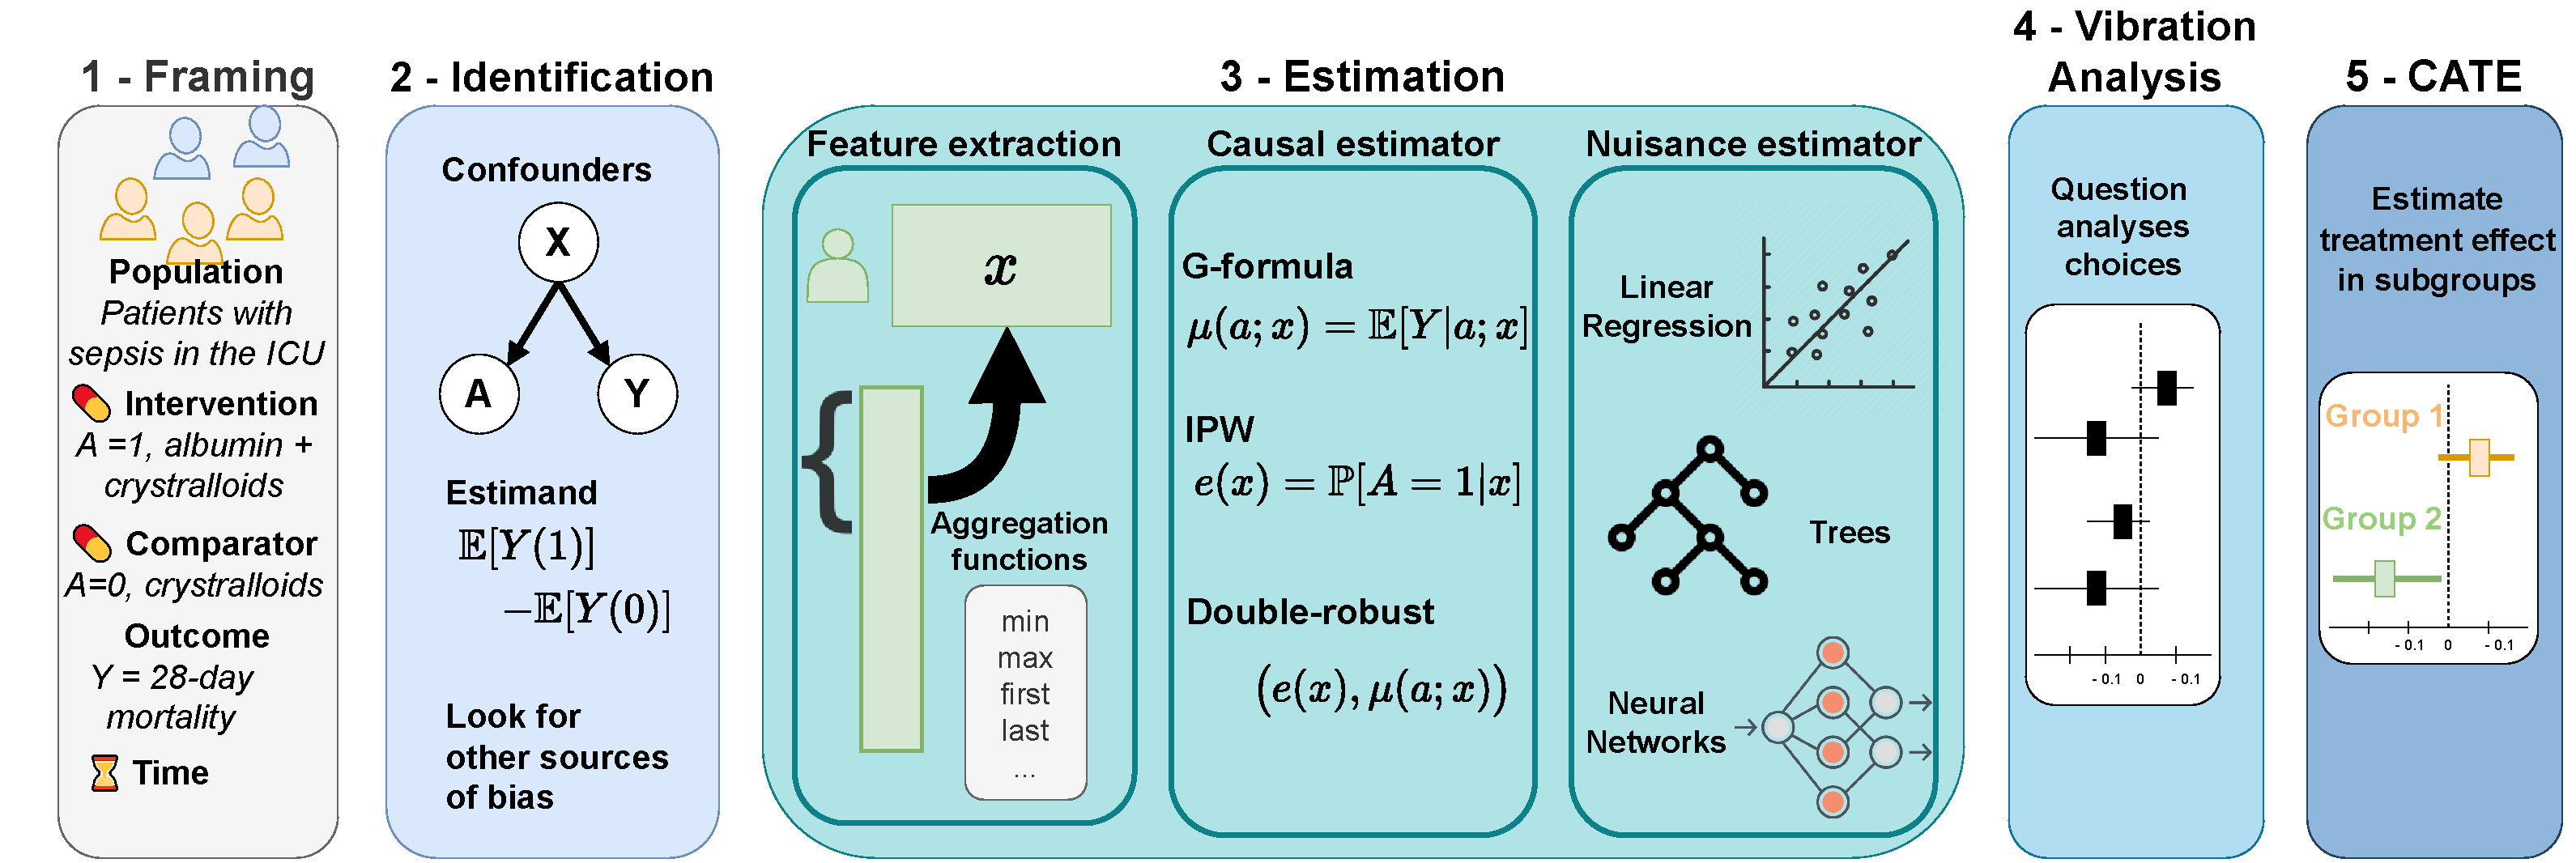
\includegraphics[width=0.9\linewidth]{img_final/complete_inference_flow.pdf}
  \caption{\textbf{Step-by-step analytic framework} -- The complete
    inference pipeline confronts the analyst with
    many choices, some guided by domain knowledge, others
    by data insights. Making those choices explicit is necessary to ensure
    robustness and reproducibility.}\label{fig:inference_framework}
\end{figure*}



Whether or not using machine learning, many pitfalls threaten an analysis'
value for decision-making. To avoid these pitfalls, we outline a simple
step-by-step analytic framework illustrated in Figure
\ref{fig:inference_framework} for retrospective case-control studies. We frame
the medical question as a target trial \cite{hernan2021methods} to match the
design to an RCT giving the gold standard average effect. Then we probe for
heterogeneity --predictions on sub-groups--  going beyond what RCTs can
achieve.

\subsection*{Step 1: study design -- Frame the question to avoid biases}\label{sec:framing}


\begin{table*}[b!]
  \resizebox{\linewidth}{!}{%
    \begin{tabular}{|l|l|l|l|}
      \hline
      \multicolumn{1}{|c|}{\textbf{PICO component}} & \multicolumn{1}{c|}{\textbf{Description}}       & \multicolumn{1}{c|}{\textbf{Notation}}                 & \multicolumn{1}{c|}{\textbf{Example}}         \\ \hline
      \cellcolor{P}\textbf{Population}              & What is the target population of interest?      & $X \sim \mathbb{P}(X)$, the covariate distribution     & \makecell[l]{Patients with sepsis in the ICU} \\ \hline
      \cellcolor{I}\textbf{Intervention}            & What is the treatment?                          & \makecell[l]{$A \sim \mathbb{P}(A=1)=p_A$,                                                             \\ the probability to be treated} & Combination of crystalloids and albumin \\ \hline
      \cellcolor{C}\textbf{Control}                 & What is the clinically relevant comparator?     & $1-A \sim 1-p_A$                                       & Crystalloids only                             \\ \hline
      \cellcolor{O}\textbf{Outcome}                 & \makecell[l]{What are the outcomes to compare?} & \makecell[l]{$Y(1), Y(0) \sim \mathbb{P}(Y(1), Y(0))$,                                                 \\ the potential outcomes distribution}  & 28-day mortality \\ \hline
      \cellcolor{T}\textbf{Time}                    & \makecell[l]{Is the start of follow-up aligned                                                                                                           \\with intervention assignment?} & \makecell[l]{N/A}  & \makecell[l]{Intervention \\ within the first day} \\ \hline
    \end{tabular}%
  }\\
  \caption{PICO(T) components help to clearly define the
    medical question of interest.}\label{table:picot}
\end{table*}


Grounding decisions on evidence needs well-framed questions, defined by their
PICO(T) components. Population, Intervention, Control, and Outcome \cite{richardson1995well,riva2012your}, and
in case of EHRs or claims data an additional time component, are necessary to
concord with a (hypothetical) target randomized clinical trial \cite{hernan_using_2016,wang2023emulation} -- Table
\ref{table:picot}.

Without care in defining these PICO(T) components, non-causal associations
between treatment and outcomes can easily be introduced into an analysis \cite{catalogofbias}. The
time-varying nature of EHR calls for checking systematically of the Population
and Time components by addressing two commonly encountered types of bias.


\paragraph{Selection Bias:} In EHRs, outcomes and treatments are often not
directly available and need to be inferred from indirect events. These signals
could be missing not-at random, sometimes correlated with the treatment
allocation \cite{weiskopf2023healthcare}. For example, billing codes can be
strongly associated with case-severity and cost. Consider comparing the
effectiveness of fluid resuscitation with albumin to crystalloids. As albumin is
more costly, this treatment is more likely to have a sepsis billing code. On the
contrary, for patients treated with crystalloids, only the most severe cases
will have a billing code. Naively comparing patients would overestimate the
effect of albumin.

\paragraph{Immortal time bias:} Improper alignment of the inclusion defining
event and the intervention time is a major source of bias in time-varying data
\cite{suissa2008immortal,hernan2016specifying,wang2022understanding}. Immortal time bias (illustrated in
Appendix \ref{apd:fig:immortal_time_bias}) occurs when the follow-up period,
i.e. cohort entry, starts before the intervention, e.g. prescription for a
second-line treatment. In this case, the treated group will be biased towards
patients still alive at the time of assignment and thus overestimating the
effect size. Other frequent temporal biases are lead time bias
\cite{Oke2021leadtimebias,fu2021timing} or right censorship  \cite{hernan2016specifying}, and attrition bias
\cite{Bankhead2017attritionbias}. Good
practices include explicitly stating the cohort inclusion event   \cite[Chapter~10:Defining Cohorts]{ohdsi2019book} and defining
an appropriate grace period between starting time and the intervention
assignment \cite{hernan2016specifying}. At this step, a population timeline can
help.


\subsection*{Step 2: identification -- List necessary information to answer the causal question}\label{sec:identification}

The identification step builds a causal model to answer the research question.
%
Indeed, the analysis must compensate for differences between
treated and non-treated that are not due to the intervention
(\cite[chapter~1]{pearl2018book},
\cite[chapter~1]{hernan2020causal}).

\paragraph{Causal Assumptions}

Valid causal inference requires assumptions  \cite{rubin2005causal} --detailed
in \nameref{apd:causal_assumptions}. The analyst should thus review the
plausibility of the following: 1) Unconfoundedness: after adjusting for the
confounders as ascertained by domain expert insight, treatment allocation should
be random; 2) Overlap --also called positivity-- the distribution of confounding
variables overlaps between the treated and controls --this is the only
assumption testable from data \cite{austin2015moving}--; 3) No interference
between units and consistency in the treatment, a reasonable assumption in most
clinical questions.

\paragraph{Categorizing covariates}
%
Potential predictors --covariates-- should be categorized depending on their
causal relations with the intervention and the outcome (illustrated in
\nameref{apd:causal_variables}): \emph{confounders} are common causes of the
intervention and the outcome; \emph{colliders} are caused by both the
intervention and the outcome; \emph{instrumental variables} are a cause of the
intervention but not the outcome, \emph{mediators} are caused by the
intervention and is a cause of the outcome. Finally, \emph{effect modifiers}
interact with the treatment, and thus
modulate the treatment effect in subpopulations \cite{attia2022proposal}.

To capture a valid causal effect, the analysis should only include confounders
and possible treatment-effect modifiers to study the resulting heterogeneity.
Regressing the outcome on instrumental and post-treatment variables (colliders
and mediators) will lead to biased causal estimates
\cite{vanderweele2019principles}. Drawing causal Directed Acyclic Graphs
(DAGs) \cite{greenland1999causal}, \emph{eg} with a webtool such as DAGitty \cite{textor2011dagitty}, helps capturing the relevant
variables and defining a suitable estimand or effect measure. The
\emph{estimand} is the final statistical quantity estimated from the data.
Depending on the question, different estimands are better suited to contrast
the two potential outcomes E[Y(1)] and E[Y(0)] \cite{imbens_nonparametric_2004,colnet2023risk}. For continuous outcomes, risk
difference is a natural estimand, while for binary outcomes (e.g. events) the
choice of estimand depends on the scale. Whereas the risk difference is very
informative at the population level, e.g. for medico-economic decision-making,
the risk ratio and the hazard ratio are more informative at the level of
sub-groups or individuals \cite{colnet2023risk}.

\subsection*{Step 3: Estimation -- Compute the causal effect of interest}\label{sec:estimation}

%\paragraph{Confounder extraction}
%
%Measured variables extracted from the raw EHRs should match the confounders
%listed in the causal graph.

\paragraph{Confounder aggregation}
Confounders captured via measures collected over multiple time points must be
aggregated at the patient level. Simple forms of aggregation include taking the
first or last value before a time point, or an aggregate such as mean or median
over time. More elaborate choices may rely on hourly aggregations providing more
detailed information on the disease course such as vital signs. They may reduce
confounding bias between rapidly deteriorating and stable patients but also
increase the number of confounders making estimation more challenging
\cite{damour2020overlap}. The increase of variance occurs either in
arbitrarily small propensity scores for treatment models or in hazardous
extrapolation from one group to another for outcome model. If multiple
choices appear reasonable, one should compare them in a vibration analysis
(see \nameref{sec:vibration_analysis}).

Beyond tabular data, unstructured clinical text may capture confounding or
prognostic information \cite{horng2017creating,jiang2023health} which can be
added in the causal model \cite{zeng2022uncovering}.
However, high-dimensional
confounder space such as text may break the positivity assumption just as hourly
aggregation choices for measurements.

\paragraph{Causal estimators or statistical modeling}

A given estimand can be estimated through different methods. One can model the
outcome with regression models also known as
G-formula, \cite{robins1986role} and use it as a predictive counterfactual model
for all possible treatments for a given patient. Alternatively, one can model
the propensity of being treated use it for matching or Inverse Propensity
Weighting (IPW) \cite{austin2015moving}. Finally, doubly robust methods model
both the outcome and the treatment, benefiting from the convergence of both
models \cite{wager2020stats}. There is a variety of doubly robust models,
reviewed in \nameref{apd:causal_estimators}.

\paragraph{Estimation models of outcome and treatment}

The causal estimators use models of the outcome or the treatment --called
nuisances. There is currently no clear best practice to choose the corresponding
statistical model \cite{wendling2018comparing, dorie2019automated}. The
trade-off lies between simple models risking misspecification of the nuisance
parameters versus flexible models risking to overfit the data at small sample
sizes. Stacking models of different complexity as in a super-learner is a good
solution to navigate the trade-off \cite{van2007super,doutreligne2023select}.

\subsection*{Step 4: Vibration analysis -- Assess the robustness of the hypotheses}\label{sec:vibration_analysis}

Some choices in the pipeline may not be clear cut. Several options should then
be explored, to derive conceptual error bars going beyond a single statistical
model. When quantifying the bias from unobserved confounders, this process is
sometimes called sensitivity analysis \cite{schneeweiss2006sensitivity,thabane2013tutorial,fda_statistical_2021}.
Following \cite{patel2015assessment}, we use the term vibration analysis to
describe the sensitivity of the results to all analytic choices.

\subsection*{Step 5: Treatment heterogeneity -- Compute treatment effects on subpopulations}\label{sec:treatment_heterogeneity}

Once the causal design and corresponding estimators are established, they can be
used to explore the variation of treatment effects among subgroups. A
causally-grounded model can be used to predict the effect of the treatment from
all the covariates --confounders and effect modifiers-- the \emph{Conditional Average
  Treatment Effect} (CATE) \cite{robertson2021assessing}. Practically, CATEs can be estimated by regressing
an individual's predictions given by the causal estimator against the sources of
heterogeneity (details in \nameref{apd:cate_results}).


\section*{Application: evidence from MIMIC-IV on which resuscitation fluid to use}%
\label{sec:application_on_mimic_iv}

We now use the above framework to extract evidence-based decision rules for
resuscitation. Ensuring optimal organ perfusion in patients with septic shock
requires resuscitation by reestablishing circulatory volume with intravenous
fluids. While crystalloids are readily available, inexpensive and safe, a
large fraction of the administered volume is not retained in the vasculature.
Colloids offer the theoretical benefit of retaining more volume, but might be
more costly and have adverse effects \cite{annane2013effects}. Meta-analyses
from multiple pivotal RCTs found no effect of adding albumin to crystalloids
\cite{xu2014comparison,li2020resuscitation} on 28-day and 90-day mortality.  Given this
previous evidence, we thus expect no average effect of albumin on mortality in
sepsis patients. However, studies --RCT \cite{caironi2014albumin}  and observational
\cite{zhou2021early}-- have
found that septic-shock patients do benefit from albumin.

\paragraph{Emulated trial: Effect of albumin in combination with crystalloids
  compared to crystalloids alone on 28-day mortality in patients with sepsis}\label{emulated_trial}

Multiple published RCTs can validate the analysis pipeline before
investigating sub-population effects for individualized decisions. Using
MIMIC-IV \cite{johnson2020mimic}, we compare the magnitude of biases introduced by reasonable
choices in the different analytical steps recalled in Figure \ref{fig:study_summary}.

\begin{figure}[h!]
  \centering
  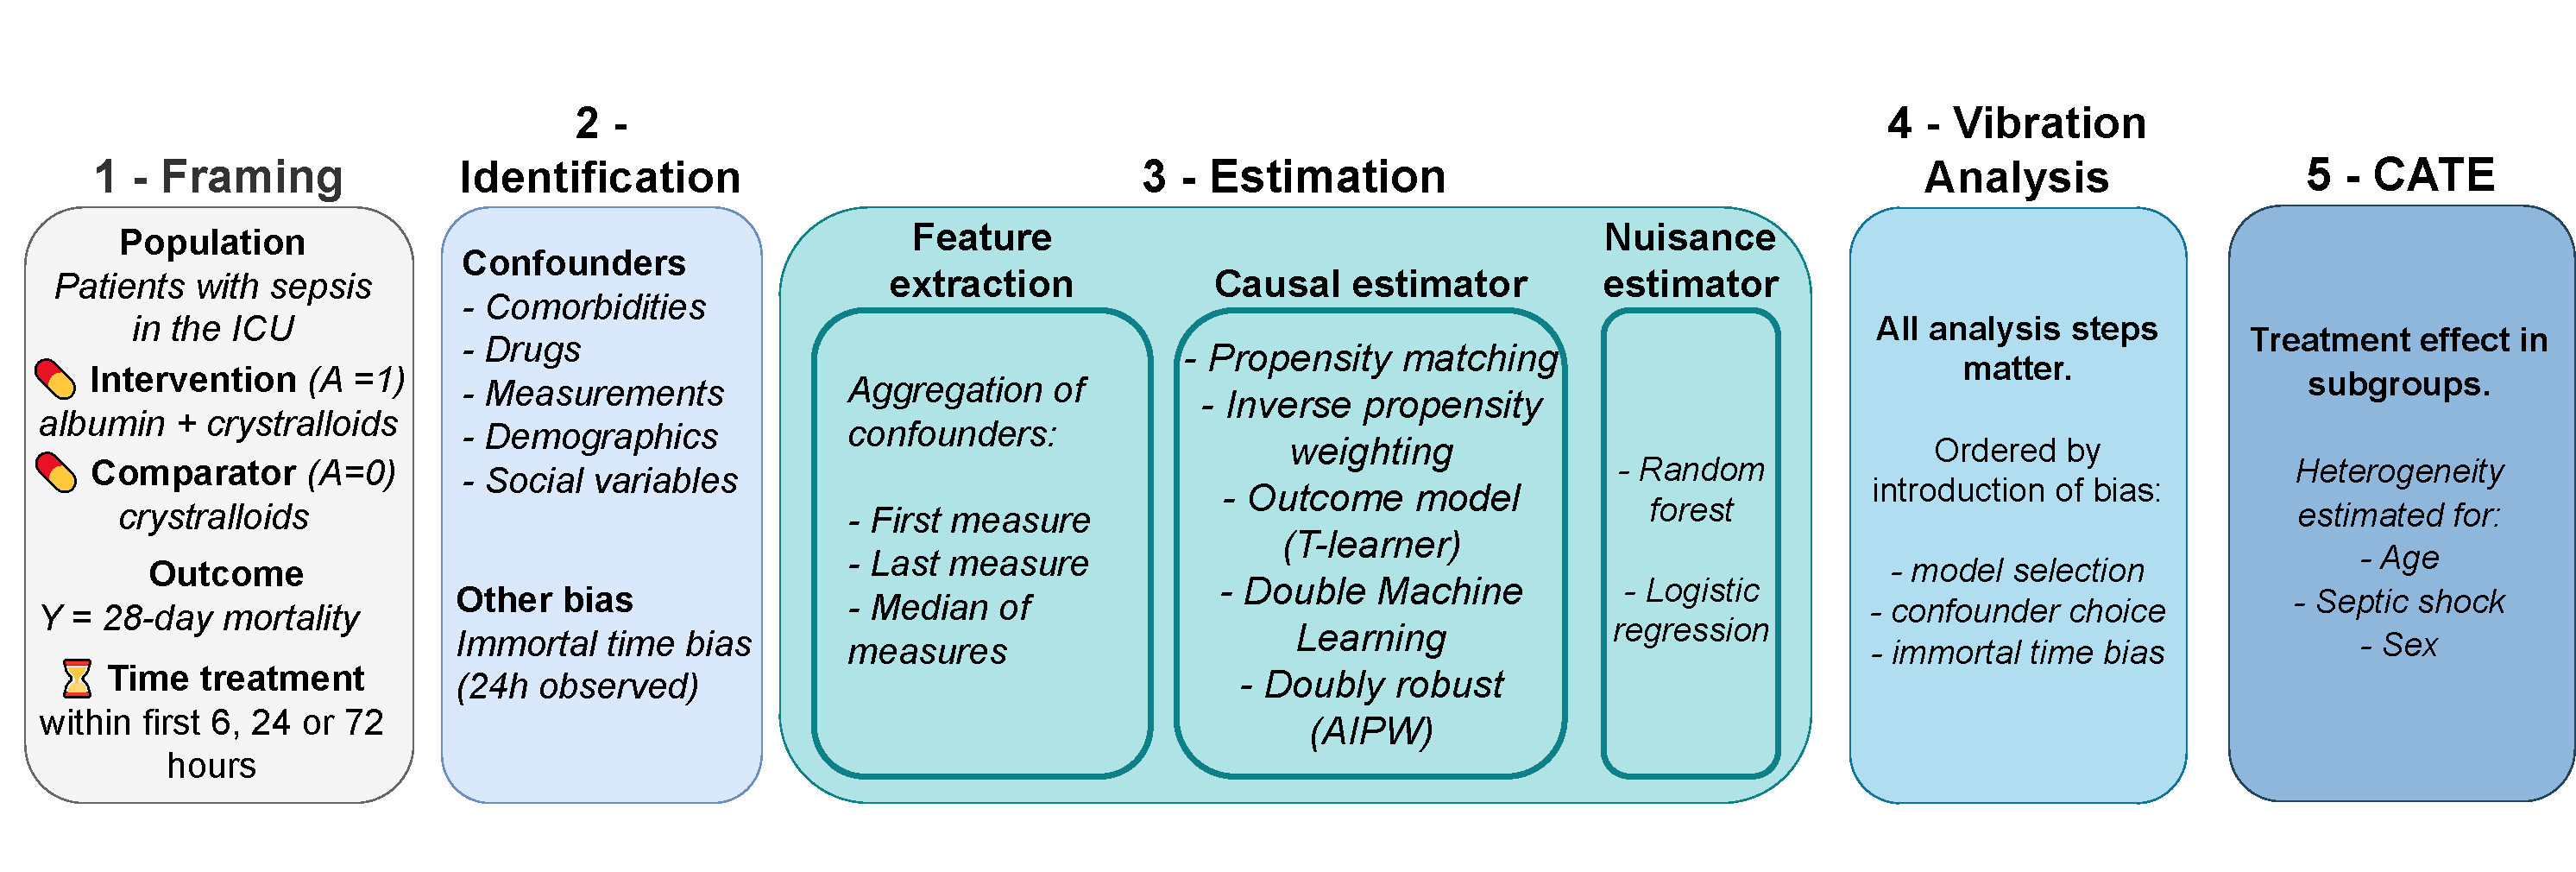
\includegraphics[width=\linewidth]{img_final/applied_inference_flow.pdf}
  \caption{\textbf{Application of the step-by-step framework on which resuscitation fluid to use.}}\label{fig:study_summary}
\end{figure}


\subsection*{Study design: effect of crystalloids on mortality in sepsis}%
\label{sec:framing_mimic_iv}

\begin{itemize}[leftmargin=2ex]
  \item \textcolor{P}{Population}: Patients with sepsis in an ICU stay
        according to the sepsis-3 definition. Other inclusion criteria:
        sufficient follow-up of at least 24 hours, and age over 18 years
        described in Appendix \ref{apd:table:albumin_for_sepsis:table1_complete}.

  \item \textcolor{I}{Intervention}: Treatment with a combination of
        crystalloids and albumin during the first 24 hours of an ICU stay.

  \item \textcolor{C}{Control}: Treatment with crystalloids only in the first 24
        hours of an ICU stay.

  \item \textcolor{O}{Outcome}: 28-day mortality.

  \item \textcolor{T}{Time}: Follow-up begins after the first administration of
        crystalloids. Thus, we potentially introduce a small immortal time bias
        by allowing a time gap between follow-up and the start of the albumin
        treatment --see the full timeline in \nameref{apd:graphical_timeline}. Because
        we are only considering the first 24 hours of an ICU stay, we
        hypothesize that this gap is insufficient to affect our results. We test
        this hypothesis in the vibration analysis step.
\end{itemize}

In MIMIC-IV, these inclusion criteria yield 18,121 patients of which 3,559 were treated with a combination of crystalloids and albumin. While glycopeptide antibiotic therapy   was similar between both groups (51.8\% crystalloid vs 51.5\% crystalloids + albumin), aminoglycosides, carbapenems, and beta-lactams were more frequent in the crystalloid only group (2.0\% vs. 0.7\%, 4.3\% vs. 2.6\%, and 35.5\% vs. 13.8\%, respectively). The crystalloid only group was more frequently admitted as an emergency (57.3\% vs. 30.7\%). Vasopressors (80.2\% vs 41.7\%) and ventilation (96.8\% vs 87.0\%) were more prevalent in the treated populations, underlying the overall higher severity of patients receiving albumin (mean SOFA at admission 6.9 vs. 5.7).
Table \ref{table:albumin_for_sepsis:table1_simple} details
patient characteristics and \nameref{apd:selection_flowchart} details the selection flowchart.


\begin{table}[h!]
  \centering\small
  \resizebox{\columnwidth}{!}{
    \begin{tabular}{llllll}
\toprule
{} & Missing &       Overall & Cristalloids only & Cristalloids + Albumin & P-Value \\
                           &         &               &                   &                        &         \\
\midrule
n                          &         &         18421 &             14862 &                   3559 &         \\
Female, n (\%)              &         &   7653 (41.5) &       6322 (42.5) &            1331 (37.4) &         \\
White, n (\%)               &         &  12366 (67.1) &       9808 (66.0) &            2558 (71.9) &         \\
Emergency admission, n (\%) &         &   9605 (52.1) &       8512 (57.3) &            1093 (30.7) &         \\
admission\_age, mean (SD)   &       0 &   66.3 (16.2) &       66.1 (16.8) &            67.3 (13.1) &  <0.001 \\
SOFA, mean (SD)            &       0 &     6.0 (3.5) &         5.7 (3.4) &              6.9 (3.6) &  <0.001 \\
lactate, mean (SD)         &    4616 &     3.0 (2.5) &         2.8 (2.4) &              3.7 (2.6) &  <0.001 \\
\bottomrule
\end{tabular}
%
  }
  \\[.5ex]

  \caption{Characteristics of the trial population measured on the first 24
    hours of ICU stay. Appendix \ref{apd:table:albumin_for_sepsis:table1_complete}
    describes all confounders used in the analysis.}\label{table:albumin_for_sepsis:table1_simple}
\end{table}


\subsection*{Identification: listing confounders}\label{sec:identification_mimic_iv}

For confounders selection we use a causal DAG shown in Figure
\ref{fig:causal_diagram_albumin}. Gray confounders are not controlled for since
they are not available in the data. However, resulting confounding biases are
captured by proxies such as comorbidity scores (SOFA or SAPS II) or other
variables (eg. race, gender, age, weight).
%
\nameref{apd:albumin_for_sepsis:table1_complete} details confounders
summary statistics for treated and controls.

\subsection*{Estimation}\label{sec:estimation_mimic_iv}


\paragraph{Confounder aggregation:}

We tested multiple aggregations such as the last value before the start of the
follow-up period, the first observed value, and both the first and last values as
separated features.

\paragraph{Causal estimators:}

We implemented multiple estimation strategies, including Inverse Propensity
Weighting (IPW), outcome modeling (G-formula) with T-Learner, Augmented Inverse
Propensity Weighting (AIPW) and Double Machine Learning (DML). We used the
python packages dowhy \cite{sharma2018tutorial} for IPW implementation and
EconML \cite{battocchi2019econml} for all other estimation strategies.
Confidence intervals were estimated by bootstrap (50 repetitions).
\nameref{apd:causal_estimators} and
\nameref{apd:packages} detail the estimators and the available Python
implementations.

\paragraph{Outcome and treatment estimators:}

To model the outcome and treatment, we used two common but different
estimators: random forests and ridge logistic regression implemented with scikit-learn
\cite{pedregosa2011scikit}. We chose the
hyperparameters with a random search procedure (\nameref{apd:hyper_parameter_search}). While logistic regression handles
predictors in a linear fashion, random forests bring the benefit of modeling
non-linear relations.


\subsection*{Vibration analysis: Comparing sources of systematic errors}%
\label{sec:vibration_analysis_mimic_iv}


\paragraph{Study design -- Illustration of immortal time bias:}

To illustrate the risk of immortal-time bias, we vary the eligibility period of
treatment or control in a shorter or longer time window than 24 hours. As
explained in \autoref{sec:framing}, a longer eligibility period means that
patients are more likely to be treated if they survived up to the intervention
and hence the study is biased to overestimate the beneficial effect of the
intervention. Figure \ref{fig:vibration:itb} shows that longer eligibility
periods lead to albumin being markedly more efficient.

\begin{figure*}[h!]
  \begin{subfigure}[b]{\linewidth}
    \caption{\bfseries Framing -- Immortal Time Bias}\label{fig:vibration:itb}
    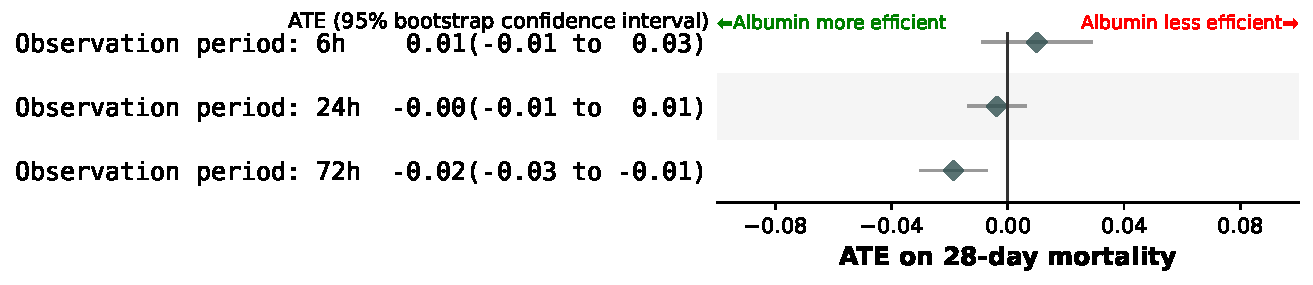
\includegraphics[width=0.765\linewidth, right]{img_final/itb__dr_forest_agg_first_last__bs_30_shared_x_axis.pdf}
  \end{subfigure}
  \vfill
  \begin{subfigure}[b]{\linewidth}
    \centering
    \caption{\bfseries Identification -- confounders choice}\label{fig:vibration:confounders}
    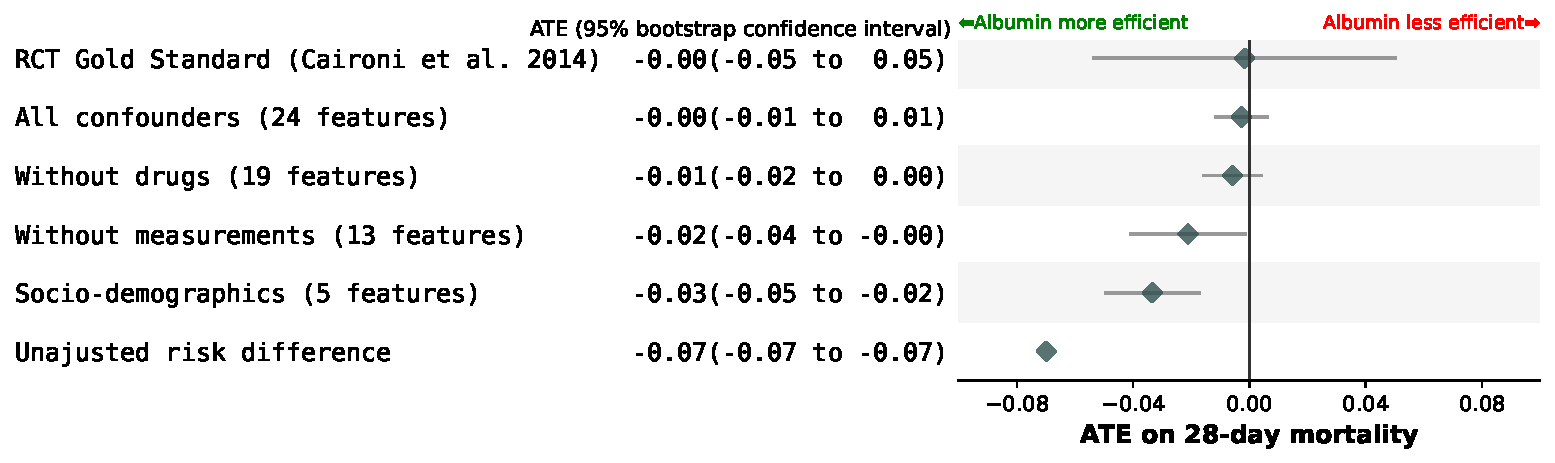
\includegraphics[width=.9\linewidth, right]{img_final/sensitivity_confounders_main_shared_x_axis.pdf}
  \end{subfigure}
  \vfill
  \begin{subfigure}[b]{\linewidth}
    \centering
    \caption{\bfseries Model selection}\label{fig:vibration:models}
    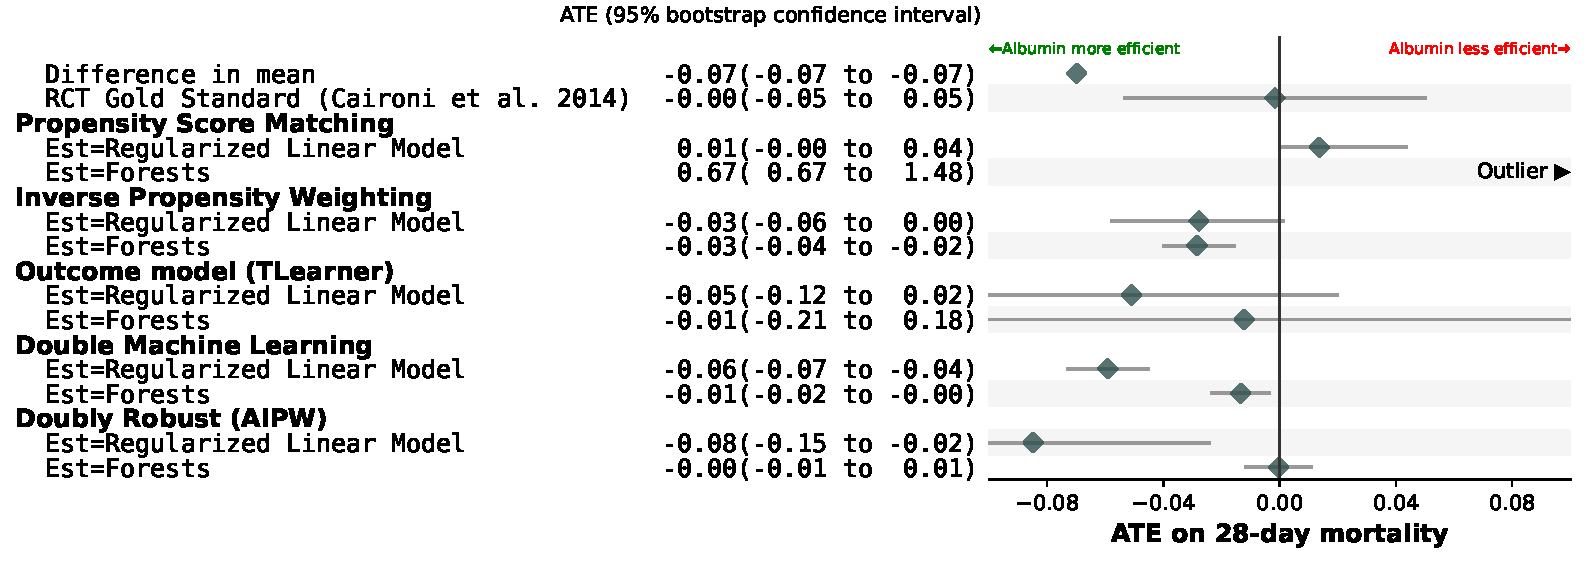
\includegraphics[width=0.891\linewidth, right]{img_final/estimates_20230712__est_lr_rf__bs_50_shared_x_axis.pdf}
  \end{subfigure}
  \vfill
  \caption{\textbf{The effect of choices on the three
      analytical steps} -- All three
    analytical steps are equally important for the validity of the analysis.
    \ref{fig:vibration:itb}) Framing step: Poor framing introduces time bias: A longer
    observation period (72h) artificially favors the efficacy of Albumin.
    \ref{fig:vibration:confounders}) Identification step: Choosing less informed confounders set
    introduces increasing bias in the results. \ref{fig:vibration:models}) Model selection step:
    Different estimators give different results. Score matching yields
    unconvincingly high estimates, inconsistent with the published RCT. With
    other causal approaches, using linear estimators for nuisances suggest a
    reduced mortality risk for albumin, while using forests for nuisance models
    points to no effect, which is consistent with the RCT gold standard.
    \\The diamonds depict the mean effect and the bar are the 95\% confidence
    intervals obtained respectively by 30, 30 and 50 bootstrap repetitions. For
    framing and identification, the estimator is a doubly robust learner (AIPW)
    with random forests for nuisances. Features are aggregated by taking the
    first and last measurements for all experiments.}\label{fig:vibration_analysis}
\end{figure*}


\paragraph{Confounder choice} We consider other choice of confounding variables
(\nameref{apd:vibration_analysis_for_confounders}). Figure
\ref{fig:vibration:confounders} shows that a less thorough choice, neglecting the
administrated drugs, makes little to no difference. Major errors, such as
omitting the biological measurements or using only socio-demographical
variables, lead to sizeable bias.

\paragraph{Estimation choices -- Confounder aggregation, causal and nuisance estimators:}

Figure \ref{fig:vibration:models} shows varying confidence intervals (CI)
depending on the method. Doubly-robust methods provide the narrowest CIs,
whereas the outcome-regression methods have the largest CI. The estimates of the
forest models are closer to the consensus across prior studies (no effect) than
the logistic regression indicating a better fit of non-linear relationships. We
only report the first and last pre-treatment feature aggregation strategy, since
detailed analysis showed little differences for other aggregations (\nameref{apd:detailed_results}). Both methodological studies \cite{naimi2023challenges} and
consistency with published RCTs suggest to prefer doubly-robust approaches.

\subsection*{Treatment heterogeneity: Which treatment for a sub-population?}%
\label{sec:treamtent_heterogeneity_mimic_iv}


With adequate choice of study design, confounding variables and causal
estimator, the average treatment effect matches well published findings:
Pooling evidence from high-quality RCTs, no effect of albumin in severe
sepsis was demonstrated for both 28-day mortality (odds ratio (OR) 0.93,
95\% CI 0.80-1.08) and 90-day mortality (OR 0.88, 95\% CI 0.761.01)
\cite{xu2014comparison}.
%
Having validated the analytical pipeline, we can use it to inform
decision-making. We explore
heterogeneity along four binary patient characteristics, displayed in Figure
\ref{fig:albumin_for_sepsis:cate_results}. We find that albumin is beneficial
with patient with septic shock consistent with one
RCT  \cite{caironi2014albumin}. It is also beneficial for older patients (age >=60) and males.

\begin{figure}[h!]
  \begin{minipage}{.4\linewidth}
    \caption{\textbf{Subgroup distributions of Individual Treatment
        effects}:
      better treatment efficacy for patients older than 60 years, septic shock,
      and to a lower extent males. The final estimator is ridge regression. The
      boxes contain the $25^\text{th}$ and $75^\text{th}$ percentiles of the CATE
      distributions with the median indicated by the vertical line. The whiskers
      extend to 1.5 times the inter-quartile range of the
      distribution.}\label{fig:albumin_for_sepsis:cate_results}
  \end{minipage}%
  \hfill%
  \begin{minipage}{.6\linewidth}
    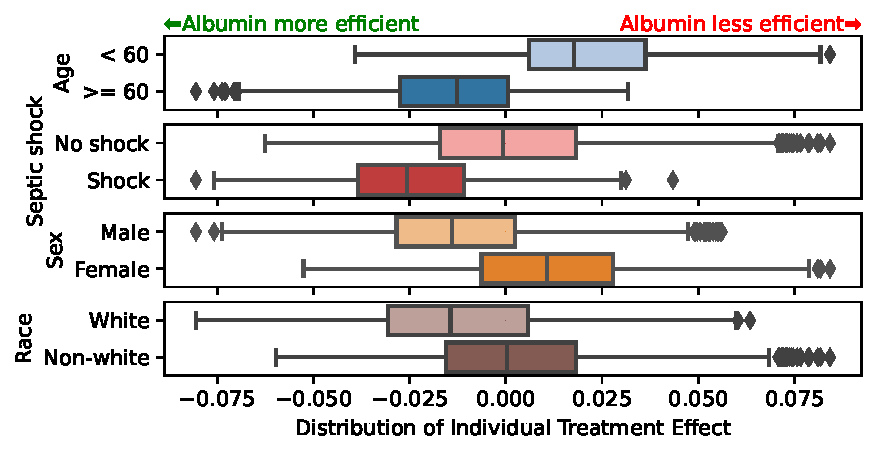
\includegraphics[width=\linewidth]{img_final/boxplot_est__DML__nuisances__Forests__final_Ridge.pdf}
  \end{minipage}%
\end{figure}


\section*{Discussion and conclusion}\label{sec:discussion}

% -	Ideas of the discussion
% o	The three steps are important, list them in simple terms, but a sentence rather than a name
% o	We argue to anchor validity by comparing the average effect to a target trial, even when the goal of the analysis is heterogeneous effect. Importance of sub-population analysis to individualize decision
% o	No magic bullet
% o     Go back to decision-making
% o	Conclusion: racial bias and equity


Valid decision-making evidence from EHR data requires a clear causal framework.
Indeed, machine-learning algorithms have often extracted non-causal associations
between the intervention and the outcome, improper for decision-making
\cite{winkler2019association,badgeley2019deep,obermeyer2019dissecting}.
Machine learning studies in medicine often rely on an implicit causal
thinking, via a good understanding of the clinical settings.
A clear framework helps making
sure nothing falls through the cracks.

We have separated three steps important for causal validity: the choice
of study design, confounders, and estimators.
%
Regarding study design, major caveats arise from the time component,
where a poor choice of inclusion time easily brings in significant bias. Regarding choice of prediction
variables, forgetting some variables that explains both the treatment
allocation and the outcome leads to confounding bias, that however
remains small when these
variables capture weak links. Regarding choice of causal estimators,
preferring flexible models such as random forests reduces the bias, in
particular for doubly-robust estimators.
%
We have shown that all these three steps are equally important: paying no
attention to one of them leads to invalid estimates of treatment effect,
yet imperfect but plausible choices lead to small biases of the same
order of magnitude for all steps.
%
For instance, despite the emphasis often put on choice of confounders,
minor deviations from the expert's causal graph did not introduce
substantial bias (\nameref{apd:vibration_analysis_for_confounders}), no larger than a too
rigid choice of estimator.


% Importance of reference target trial
To assert the validity of the analysis, we argue to relate as much as
possible the average effect to a reference target trial, even when the
goal is to capture the heterogeneity of the effect to individualize
decisions.
% Go back to decision-making
EHRs complement RCTs: RCTs cannot address all the
subpopulations and local practices
\cite{travers2007external,kennedy2015literature}. EHRs often cover many
individuals, with the diversity needed to model treatment
heterogeneity. The corresponding model can then inform better
decision-making \cite{prosperi2020causal}: a sub-population analysis  (as in Figure
\ref{fig:albumin_for_sepsis:cate_results}) can distill rules on which groups
of patients should receive a treatment. Beyond a sub-group perspective,
patient-specific estimates facilitate a personalized approach
to clinical decision-making \cite{kent2018personalized}.
%
% No magic bullet and its not all about ML

Even without considering a specific intervention, anchoring
machine-learning models on
causal mechanisms can make them more robust to distributional shift \cite{scholkopf2021toward},
thus safer and fairer for clinical use
\cite{richens2020improving,plecko2022causal}.
%
Yet it is important to keep in mind that better prediction is not per se
a goal in healthcare.
%
Establishing strong predictors might be less important than identifying
moderately strong but modifiable risk factors as established in the Framingham
cohort \cite{brand1976multivariate}, while others such as the QRISK score are used to optimize population-wide cost-effectiveness, but not individual treatment effect.

No sophisticated data-processing tool can safeguard against
invalid study design or a major missing confounder, loopholes that can
undermine decision-making systems. Our framework helps the investigator
ensure
causal validity by outlining the important steps and relating average effects to
RCTs. Causal grounding of individual predictions should reduce the social
disparities that they reinforce
\cite{rajkomar2018ensuring,mitra2022future,ehrmann2023making}, as these are driven by
historical decisions and not biological mechanisms. At the population
level, it leads to better public health decisions. For instance, going
back to cardio-vascular diseases, the stakes are to go beyond risk
scores and also account for responder status when prescribing prevention
drugs.


\section*{Availability of data and materials}

The datasets are available on PhysioNet (
\url{https://doi.org/10.13026/6mm1-ek67}). We used MIMIC-IV.v2.2 The code for
data preprocessing and analyses are available on github
\url{https://github.com/soda-inria/causal_ehr_mimic/}.

% \section*{Fundings}
% This study was supported by an unrestricted educational grants to TS (Swiss
% National Science Foundation, P400PM\_194497 / 1) as well as an ERC grant to GV
% (Intercept-T2D HORIZON-HLTH-2022-STAYHLTH-02-01). LAC is funded by the National
% Institute of Health through NIBIB R01 EB017205.

\section*{Authors contributions}

MD and TS designed the study, MD performed the analysis and wrote the manuscript.
TS, JA, CM, LAC, GV reviewed and edited the manuscript.

% \section*{Competing interests}

% All authors declare no financial or non-financial competing interests.
\clearpage

\section*{Supporting information}

% Include only the SI item label in the paragraph heading. Use the \nameref{label} command to cite SI items in the text.
\paragraph*{S1 Fig.}
\label{apd:motivating_example}
{\bf Motivating example: Failure of predictive models to predict mortality
  from pretreatment variables.}
To illustrate how machine learning frameworks can fail to inform decision
making, we present a motivating example from MIMIC-IV. Using the same
population and covariates as in the main analysis (described in Table
\ref{apd:table:albumin_for_sepsis:table1_complete}), we train a predictive
model for 28-day mortality. We split the data into a training set (80\%) and a
test set (20\%). The training set uses the last measurements from the first 24
hours, whereas the validation set only uses the last measurements before the
administration of crystalloids. We split the train set into a train and a
validation set. We fit a HistGradientBoosting classifier
\footnote{\url{https://scikit-learn.org/stable/modules/ensemble.html\#histogram-based-gradient-boosting}}
on the train set and evaluate the performance on the validation set and on the
test set. We see good area under the Precision-recall curve (PR AUC) on the
validation set, but a deterioration of 10 points on the test set (Figure
\ref{apd:fig:motivating_example_pr_auc}). The same is seen in Figure
\ref{apd:fig:motivating_example_roc_auc} when measuring performances with Area
Under the Curve of the Receiving Operator Characteristic (ROC AUC). On the
contrary, a model trained on pre-treatment features yields competitive
performances. This failure illustrates well the shortcuts on which predictive
models could rely to make predictions. A clinically useful predictive model
should support decision-making --in this case, addition of albumin to
crystalloids-- rather than maximizing predictive performance. In this example,
causal thinking would have helped to identify the bias introduced by
post-treatment features. In fact, these features should not be included in a
causal analysis since they are post-treatment colliders.

This kind of error might sound naive to a clinical expert but relying on
shortcuts --some of them being post-treatment variables-- is a common error.
Here, we detail some real use cases where machine learning fail in providing
useful predictions for decision-making. \cite{badgeley2019deep} use deep
learning to predict hip fracture using confounding patient and healthcare
variables. An example of such covariates shown by the authors is the triage of
patients before imaging that results in the model trying to predict the image
acquisition machine and rely on it to predict hip fracture.
\cite{obermeyer2019dissecting} describe the use of algorithm in US extra-care
programs. By equating care needs with previous care costs (in a pure
predictive fashion), the algorithm falsely conclude that Black patients are
healthier than equally white patients, since they do less money is spent on
them for a given level of need. Beyond Machine Learning, we also spotted the
inclusion of post-treatment variables in the development of the recent SCORE2
cardio-vascular risk score \cite{score22021score2}: \emph{Our risk models
  might have underestimated CVD risk be- cause data used to estimate multipliers
  were likely to include some people already on CVD prevention therapies (e.g.
  statins or anti- hypertensive medication}. This score might be used to inform
on the initiation of statins for primary prevention. But, relying on
post-treatment, it might under-discover patients who would benefit from
statins at screening time.


\begin{figure}[!h]
  \begin{subfigure}{\linewidth}
    \centering
    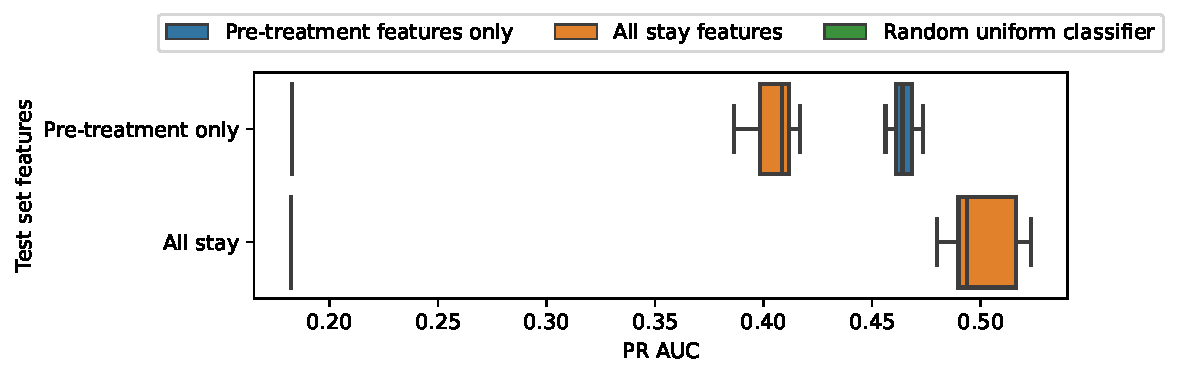
\includegraphics[width=0.8\linewidth]{img_final/predictive_failure__pr_auc.pdf}
    \caption{Area under the Precision-Recall curve (PR\_AUC)}\label{apd:fig:motivating_example_pr_auc}
  \end{subfigure}
  \hfill
  \begin{subfigure}{\linewidth}
    \centering
    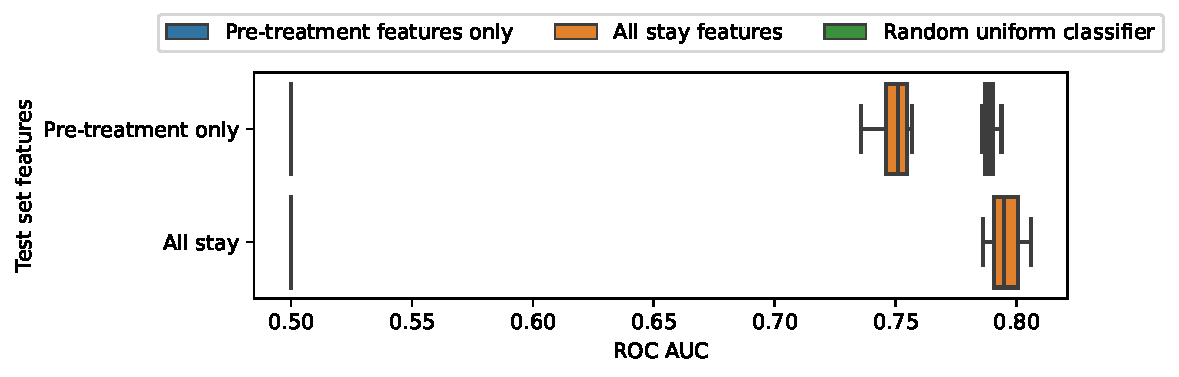
\includegraphics[width=0.8\linewidth]{img_final/predictive_failure__roc_auc.pdf}
    \caption{Area under the Receiving Operator Characteristic (ROC\_AUC)}\label{apd:fig:motivating_example_roc_auc}
  \end{subfigure}
  \caption{Failure to predict 28-day mortality from a model fitted on
    pre-treatment variables. The model is trained on the last features from
    the whole stay and tested on two validation sets: one with all stay
    features and one with last features before crystalloids administration
    (Pre-treatment only). The all-stay model performance markedly decreases in
    the pre-treatment only dataset.}\label{apd:fig:motivating_example}
\end{figure}
\clearpage


\paragraph*{S2 Fig.}
\label{apd:immortal_time_bias}
{\bf Immortal time bias illustration.}

Figure \ref{apd:fig:immortal_time_bias} illustrates the immortal time bias.
This time bias is a major pitfall in the retrospective evaluation of
screening programs  \cite{bretthauer2013principles}.

\begin{figure}[!h]
  % \begin{minipage}{.25\linewidth}
  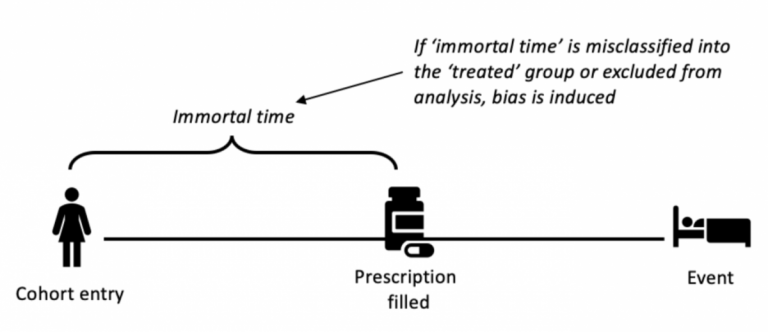
\includegraphics[width=0.7\linewidth]{img_final/catalog_of_bias_immortal_time_bias.png}
  \caption{Poor experimental design can introduce Immortal time bias, which
    leads to a treated group with falsely longer longevity
    \cite{lee2020immortaltimebias}.}\label{apd:fig:immortal_time_bias}
  % \end{minipage}%
  % \hfill%
  % \begin{minipage}{.7\linewidth}
  % \end{minipage}
\end{figure}
\clearpage


\paragraph*{S3 Fig.}
\label{apd:graphical_timeline}
{\bf Graphical timeline.}
Drawing a graphical timeline as the one in Figure
\ref{fig:cohort_timeline_albumin} during the study design helps to detect and
prevent time-related biases.

\begin{figure}[h!]
  \centering
  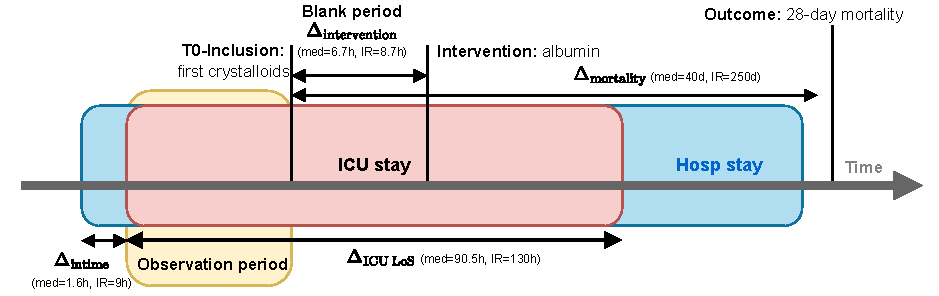
\includegraphics[width=\linewidth]{img_final/timeline_albumin_for_sepsis.pdf}
  \caption{Defining the inclusion event, the starting time T0 for follow-up, the
    intervention's assignment time and the observation window for confounders is
    crucial to avoid time and selection biases. In our study, the gap
    between the intervention and the inclusion is small
    compared to the occurrence of the outcome to limit immortal time bias: 6.7 hours vs 40
    days for mortality.\label{fig:cohort_timeline_albumin}}
\end{figure}
\clearpage


\paragraph*{S4 Fig.}
\label{apd:causal_variables}
{\bf Types of causal variables.}

Figure \ref{fig:causal_variables} illustrates the different types of causal variables.

\begin{figure}[h!]
  \begin{minipage}[t]{0.32\linewidth}
    \centering
    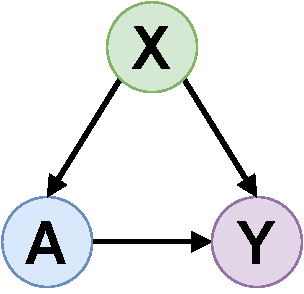
\includegraphics[width=0.72\linewidth]{img_final/confounder.pdf}
    \small\sffamily Confounder
  \end{minipage}
  \hfill
  \begin{minipage}[t]{0.32\linewidth}
    \centering
    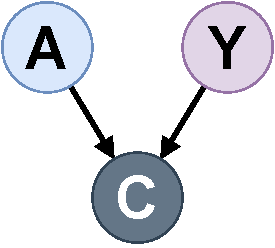
\includegraphics[width=0.72\linewidth]{img_final/collider.pdf}
    \small\sffamily Collider
  \end{minipage}
  \hfill
  \begin{minipage}[t]{0.32\linewidth}
    \centering
    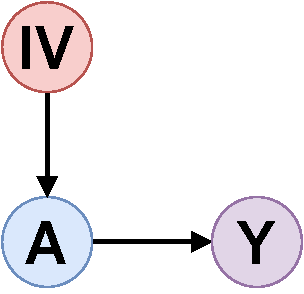
\includegraphics[width=0.72\linewidth]{img_final/instrumental_variable.pdf}
    \small\sffamily Instrumental \\variable
  \end{minipage}
  \vfill
  \begin{minipage}[t]{0.4\linewidth}
    \centering
    
\includegraphics[width=.9\linewidth]{img_final/mediator.pdf}%
    \\
    \small\sffamily Mediator
  \end{minipage}
  \hfill
  \begin{minipage}[t]{0.4\linewidth}
    \centering
    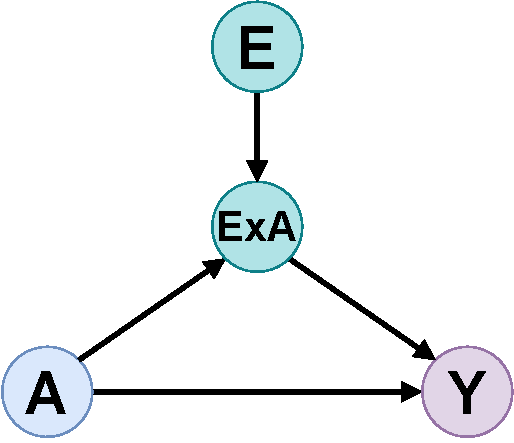
\includegraphics[width=\linewidth]{img_final/effect_modifier.pdf}%
    % \llap{%
    %   \raisebox{.555\linewidth}{\colorbox{black!10}{\parbox{1.9\linewidth}{%
    %         \sffamily\small\hspace*{-1.3ex}%
    %         \begin{tabular}{r@{\hskip 1ex}lr@{\hskip 1ex}l}
    %           A:  & Treatment                    & Y: & Outcome         \\
    %           X:  & Confounder                   & C: & Collider        \\
    %           IV: & Instrumental va\rlap{riable}                        \\
    %           M:  & Mediator                     & E: & Effect modifier \\
    %         \end{tabular}%
    %         \vspace*{-.3ex}
    %       }}\hspace*{.84\linewidth}%
    %   }}
    \small\sffamily Effect modifier \scriptsize\\Represented
    following \cite{attia2022proposal}
  \end{minipage}
  \caption{The five categories of causal variables needed for our framework: A:
    Treatment, X: Confounder, IV: Instrumental variable, M: mediator, Y:
    Outcome, C: Collider, E: Effect modifier.}\label{fig:causal_variables}
\end{figure}
\clearpage



\paragraph*{S1 Appendix.}
\label{apd:ate_on_mimic}
{\bf Estimation of Treatment effect with MIMIC data.}

We searched for causal inference studies in MIMIC using PubMed and Google
scholar with the following search terms ((MIMIC-III OR MIMIC-IV) AND (causal
inference OR treatment effect)). We retained eleven treatment effect studies
clearly following the PICO framework:

\begin{itemize}[leftmargin=2ex]
  \item \cite{liu2021effects} studied the effect of \textcolor{I}{High-flow
          nasal cannula oxygen (HFNC)} against \textcolor{C}{noninvasive
          mechanical ventilation} on \textcolor{P}{801 patients with hypoxemia
          during ventilator weaning} on \textcolor{O}{28-day mortality}. They
        used propensity score matching, and found non-negative effects as
        previous RCTs reported --though those were focused on reintubation as the
        main outcome \cite{stephan2015high,hernandez2016effect}.

  \item \cite{yarnell2023oxygenation} studied the effect of \textcolor{I}{lower hypoxemia} vs \textcolor{C}{higher
        hypoxemia thresholds for the initiation of invasive ventilation} (defined with saturation-to-inspired oxygen ratio (SF)) for
        \textcolor{P}{3,357 patients from MIMIC receiving inspired oxygen fraction greater than 0.4} on \textcolor{O}{28-day
          mortality}. Using bayesian G-computation (time-varying treatment model with
        gaussian process and outcome-model with BART, taking the treatment model as
        entry), they found protective effects for initialization at low hypoxemia.
        However, when externally validation their findings in the AmsterdamUMCdb dataset,
        they found the highest mortality probability for patients with low hypoxemia.
        Authors concluded that their model was heavily dependent on clinical context
        and baseline characteristics. There might be some starting-time bias in this study since it is really close

  \item \cite{hsu2015association} studied the effect of \textcolor{I}{indwelling
          arterial catheters (IACs)} vs \textcolor{C}{non-IAC} for
        \textcolor{P}{1,776 patients who are mechanically ventilated and did
          not require vasopressor support} on \textcolor{O}{28-day mortality}.
        They used propensity score matching and found no effect. A notebook based on google cloud access to MIMIC-IV
        replicating the study is available \href{https://github.com/alistairewj/mimic-iv-aline-study/blob/main/mimic_iv_aline.ipynb}{here}.

  \item \cite{feng2018transthoracic} studied the effect of
        \textcolor{I}{transthoracic echocardiography} vs \textcolor{C}{no
          intervention} for \textcolor{P}{6,361 patients with sepsis} on
        \textcolor{O}{28-day mortality}. They used IPW, PSM, g-formula and a
        doubly robust estimation. The propensity score was modeled with boosting
        and the outcome model with a logistic regression. They
        found a significant positive reduction of mortality (odd ratio 0.78, 95\% CI 0.68-0.90).
        \href{https://github.com/nus-mornin-lab/echo-mimiciii}{Study code is
          open source}.

  \item \cite{gani2023structural} studied the effect of \textcolor{I}{liberal
          --target SpO2 greater than 96\%--} vs \textcolor{C}{conservative
          oxygenation --target SpO2 between 88-95\%--} in \textcolor{P}{4,062
          mechanically ventilated patients} on \textcolor{O}{90-day mortality}.
        They found an advantage of the liberal strategy over liberal
        (ATE=0.13) by adjusting on age and apsii. This is not consistent with
        previous RCTs where no effects have been reported \cite{panwar2016conservative, mackle2019conservative}.

  \item \cite{shahn2020fluid} studied the effect of \textcolor{I}{fluid-limiting
          treatment --caped between 6 and 10 L--} vs \textcolor{C}{no cap on
          fluid administration} strategies for \textcolor{P}{1,639 sepsis
          patients} on \textcolor{O}{30 day-mortality}. Using a dynamic Marginal
        Structural Model with IPW, they found a protective effect of
        fluid-limitation on ATE -0.01 (95\%CI -0.016, -0.03). This is somehow
        concordant with the RIFTS RCT that found no effect of fluid limitation
        \cite{corl2019restrictive} and two previous meta-analyses
        \cite{malbrain2014fluid,meyhoff2020lower}.

  \item \cite{chinaeke2021impact} studied the effect of \textcolor{I}{statin use
          prior to ICU admission} vs \textcolor{C}{absence of pre-ICU
          prescription} for \textcolor{P}{8,200 patients with sepsis} on
        \textcolor{O}{30-day mortality}. Using AIPW (no estimator reported)
        and PSM (logistic regression), they found a decrease on mortality (ATE
        -0.039, 95\%CI -0.084, -0.026). This partly supports previous
        findings in Propensity Matching bases observational studies
        \cite{lee2017preadmission,kyu2019preadmission}. But all RCTs
        \cite{national2014rosuvastatin,singh2017effects} found no improvement for sepsis (not
        pre-admission administration though). The \cite{wan2014effect}
        meta-analysis concludes that there is lack of evidence for the use of
        statins in sepsis with inconsistent results between RCTs (no effect)
        and observational studies (protective effect).
  \item \cite{adibuzzaman2019323} studied the effect of \textcolor{I}{higher} vs
        \textcolor{C}{lower positive end-expiratory pressures (PEEP)} in
        \textcolor{P}{1,411 patients with Acute Respiratory Distress Syndrome
          (ARDS) syndrome} on \textcolor{O}{30 day mortality}. Very few details on
        the methods were reported, but they found a protective effect for higher PEEP
        consistent results from a target trial \cite{national2004higher}.
  \item \cite{adibuzzaman2019323} also studied the effect of \textcolor{I}{early
          use of a neuromuscular blocking agent } vs \textcolor{C}{placebo} in
        \textcolor{P}{752 patients moderate-severe ARDS} on \textcolor{O}{30
          day mortality}. Very few details on the methods were reported, but they found a
        protective effect for the use of a neuromuscular blocking agent,
        consistent with the results from a target trial
        \cite{papazian2010neuromuscular}.
  \item \cite{zhou2021early} studied the administration of \textcolor{I}{a
          combination of albumin within the first 24-h after crystalloids} vs
        \textcolor{C}{crystalloids alone} for \textcolor{P}{6,641 patients
          with sepsis} on \textcolor{O}{28-day mortality}. Using PSM, they found
        protective effect of combination on mortality, but insist on the
        importance of initialization timing. This is consistent with \cite{xu2014comparison}, who
        found a non-significant trend
        in favor of albumin used for severe sepsis patients and a significant
        reduction for septic shock patients, both on 90-day mortality. These
        results are aligned with \cite{caironi2014albumin} that found no effect
        for severe sepsis patient but positive effect for septic shock patients.
  \item \cite{wang2023early} studied \textcolor{I}{early enteral nutrition (EN)
          --<=53 ICU admission hours--} vs \textcolor{C}{delayed EN} for
        \textcolor{P}{2,364 patients with sepsis and EN} on
        \textcolor{O}{acute kidney injury}. With PSM, IPW and g-formula
        (logistic estimator each time), they found a protective effect
        (OR 0.319, 95\%CI 0.245, 0.413) of EEN.
\end{itemize}

These eleven studies mainly used propensity score matching (6) and IPW (4), two of
them used doubly robust methods, and only one included a non-linear estimator in
either the outcome or the treatment model. None of them performed a vibration
analysis on confounder selection or feature transformations. They have a
strong focus on patients with sepsis. Only four of them found concordant results with
previous RCTs \cite{liu2021effects,shahn2020fluid,adibuzzaman2019323}.
\clearpage


\paragraph*{S2 Appendix.}
\label{apd:causal_assumptions}
{\bf Assumptions: what is needed for causal inference from observational studies.}


The following four assumptions, referred as strong ignorability, are
needed to assure identifiability of the causal estimands with observational
data with most causal-inference methods \cite{rubin2005causal}, in
particular these we use:

\begin{assumption}[Unconfoundedness]\label{assumption:ignorability}
  \begin{equation}\label{eq:ignorability}
    \{Y(0), Y(1) \} \indep A | X
  \end{equation}
  This condition --also called ignorability-- is equivalent to the conditional
  independence on the propensity score $e(X)=\mathbb P(A=1|X)$ \cite{rosenbaum1983central}: $\{Y(0), Y(1) \}\indep  A | e(X)$.
\end{assumption}


\begin{assumption}[Overlap, also known as Positivity]\label{assumption:overlap}
  \begin{equation}\label{eq:overlap}
    \eta < e(x) < 1 - \eta \quad \forall x \in \mathcal{X} \text{ and some }   \eta > 0
  \end{equation}
  The treatment is not perfectly predictable. Or in other words, every
  patient has a chance to be treated and not to be treated. For a given set of
  covariates, we need examples of both to recover the ATE.
\end{assumption}

As noted by \cite{damour2020overlap}, the choice of covariates $X$ can
be viewed as a trade-off between these two central assumptions. A bigger
covariate set generally reinforces the ignorability assumption. In the
contrary, overlap can be weakened by large $\mathcal{X}$ because of the
potential inclusion of instrumental variables: variables only linked to the treatment which
could lead to arbitrarily small propensity scores.

% remark: There is a major counter example to these colliders (variables which
% are caused by both the outcome and the treatment),

\begin{assumption}[Consistency]\label{assumption:consistency} The observed
  outcome is the potential outcome of the assigned treatment:
  \begin{equation}\label{eq:consistancy}
    Y = A \, Y(1) + (1-A) \, Y(0)
  \end{equation}
  Here, we assume that the intervention $A$ has been well defined. This
  assumption focuses on the design of the experiment. It clearly states the link
  between the observed outcome and the potential outcomes through the
  intervention \cite{hernan2020causal}.
\end{assumption}

\begin{assumption}[Generalization]\label{assumption:generalization} The training
  data on which we build the estimator and the test data on which we make the
  estimation are drawn from the same distribution, also known as
  the ``no covariate shift'' assumption \cite{jesson2020identifying}.
\end{assumption}
\clearpage



\paragraph*{S3 Appendix.}
\label{apd:causal_estimators}
{\bf Major causal-inference methods: When to use which estimator?}


\textbf{G-formula} also called conditional mean regression
\cite{wendling2018comparing}, g-computation \cite{robins1986role}, or
Q-model \cite{snowden2011implementation}. This approach is directly modeling
the outcome, also referred to as the response surface: $\mu_{(a)}(x)
  =\mathbb{E}\left(Y \mid A=a, \mathbf{X}=x\right)$

Using an outcome estimator to learn a model for the response surface $\hat
  \mu$ (eg. a linear model), the ATE estimator is an average over the n samples:
\begin{equation}
  \hat{\tau}_G(f) = \frac{1}{n} \sum_{i=1}^n \hat \mu(x_i, 1) - \hat \mu(x_i, 0) = \frac{1}{n} \sum_{i=1}^n \hat \mu_{(1)}(x_i) - \hat \mu_{(0)}(x_i)
\end{equation}

This estimator is unbiased if the model of the conditional response surface
$\hat \mu_{(a)}$ is well-specified. This approach assumes than $Y(a) =
  \mu_a(X) + \epsilon_a$ with $\mathbb E[\epsilon|X] = 0$. The main drawback is
the extrapolation of the learned outcome estimator from samples with similar
covariates X but different intervention A.\\

\textbf{Propensity Score Matching (PSM)} To avoid confounding bias, the
ignorability assumption \ref{assumption:ignorability}) requires to contrast
treated and control outcomes only between comparable patients with respect to
treatment allocation probabilities. A simple way to do this is to group
patients into bins, or subgroups, of similar confounders and contrast the two
population's outcomes by matching patients inside these bins
\cite{stuart2010matching}. However, the number of confounder bins grows
exponentially with the number of variables. \cite{rosenbaum1983central} proved
that matching patients on the individual probabilities to receive treatment
--propensity scores-- is sufficient to verify ignorability. PSM is a
conceptually simple method, but has delicate parameters to tune such as
choosing a model for the propensity score, deciding what is the maximum
distance between two potential matches (the caliper width), the number of
matches by sample, and matching with or without replacement. It also prunes data
not meeting the caliper width criteria, and suffers from high estimation
variance in highly-dimensional data where extreme propensity weights are common.
Finally, the simple bootstrap confidence intervals are not theoretically
grounded \cite{abadie2008failure} making PSM more difficult
to use for applied practitioners.\\

\textbf{Inverse Propensity Weighting (IPW)}

A simple alternative to propensity score matching is to weight the outcome by
the inverse of the propensity score \cite{austin2015moving}. It relies on a
similar idea as matching but automatically builds a balanced population by
reweighting the outcomes with the propensity score model $\hat{e}$ to estimate
the ATE:
\begin{equation}
  \hat \tau_{IPW}(\hat e) = \frac{1}{n} \sum_{i=1}^N \frac{A_i Y_i}{\hat e(X_i)} - \frac{(1-A_i)Y_i}{(1-\hat e(X_i))}
\end{equation}

This estimate is unbiased if $\hat e$ is well-specified. IPW suffers from high
variance if some weights are too close to 0 or 1. In high dimensional cases
where poor overlap between treated and control is common, one can clip extreme
weights to limit estimation instability.\\


\textbf{Doubly Robust Learning, DRL} also called Augmented Inverse
Probability Weighting (AIPW) \cite{robins1994estimation}.

The underlying idea of DRL is to combine the G-formula and IPW estimators to
protect against a mis-specification of one of them. It first requires to
estimate the two nuisance parameters: a model for the intervention $\hat{e}$
and a model for the outcome $f$. If one of the two nuisance is unbiased, the
following ATE estimator is as well:

$$\begin{aligned} \widehat{\tau}_{A I P W}=\frac{1}{n}
    \sum_{i=1}^{n}\left(\hat \mu_{(1)}\left(x_{i}\right)-\hat \mu_{(0)}\left(x_{i}\right)+a_{i}
    \frac{y_{i}-\hat \mu_{(1)}\left(x_{i}\right)}{\hat{e}\left(x_{i}\right)}-\left(1-a_{i}\right)
    \frac{y_{i}-\hat \mu_{(0)}\left(x_{i}\right)}{1-\hat{e}\left(x_{i}\right)}\right)
  \end{aligned}$$

Moreover, despite the need to estimate two models, this estimator is more
efficient in the sense that it converges quicker than single model estimators
\cite{wager2020stats}. For this propriety to hold, one need to fit and apply
the two nuisance models in a cross-fitting manner. This means that we split
the data into K folds. Then for each fold, we fit the nuisance models on the
K-1 complementary folds, and predict on the remaining fold.

To recover Conditional Treatment Effects from the AIPW estimator,
\cite{foster2019orthogonal} suggested to regress the Individual Treatment
Effect estimates from AIPW on potential sources of heterogeneity $X^{cate}$:
$\hat tau = \argmin_{\tau \in \Theta} (\hat \tau_{AIPW}(X) - \tau(X^{cate}))$
for $\Theta$ some class of model (eg. linear model).\\

\textbf{Double Machine Learning} \cite{chernozhukov2018double} also known
as the R-learner \cite{nie2021quasi}. It is based on the R-decomposition,
\cite{robinson1988root}, and the modeling of the conditional mean outcome,
$m(x)=\mathbb E[Y|X=x]$ and the propensity score, $e(x)=\mathbb E[A=1|X=x]$:
\begin{equation}\label{eq:r_decomposition}
  y_{i}-m\left(x_{i}\right)=\left(a_{i}-e\left(x_{i}\right)\right) \tau\left(x_{i}\right)+\varepsilon_{i} \quad \text{with} \; \varepsilon_{i}=y_{i}-\varepsilon\left[4_{i} \mid x_{i}, a_{i}\right]
\end{equation}
Note that we can impose that the conditional treatment effect $\tau(x)$ only
relies on a subset of the features, $x^{cate}$ on which we want to study
treatment heterogeneity.

From this decomposition, we can derive an estimation of the ATE $\tau$, where
the right hand-side term is the empirical R-Loss:
\begin{align}\label{eq:r_loss}
  \hat{\tau}(\cdot)=\operatorname{argmin}_{\tau}\left\{\frac{1}{n} \sum_{i=1}^{n}\left(\left(y_{i}-m\left(x_{i}\right)\right)-\left(a_{i}-e(x_{i})\right) \tau\left(x^{cate}_{i}\right)\right)^{2}\right\}
\end{align}

The full procedure for R-learning is first to fit the nuisances: $\hat m$ and
$\hat e$. Then, minimize the estimated R-loss eq.\ref{eq:r_loss}, where
the oracle nuisances $(e, m)$ have been replaced by their estimated
counterparts $(\hat e, \hat m)$. Minimization can be done by regressing
the outcome residuals weighted by the treatment residuals. Finally, get
the ATE by averaging conditional treatment effect $\tau(x^{cate})$ over
the population.

This estimator has also the doubly robust proprieties described for AIPW. it
should have less variance than AIPW since it does not use the propensity score
in the denominator.
\clearpage


\paragraph*{S4 Appendix.}
\label{apd:statistical_considerations}
{\bf Statistical considerations when implementing
  estimation.}

\textbf{Counterfactual prediction lacks off-the-shelf cross-fitting estimators}

Doubly robust methods use cross-fit estimation of the nuisance parameters,
which is not available off-the-shelf for IPW and T-Learner estimators. For
reproducibility purposes, we did not reimplement internal cross-fitting for
treatment or outcome estimators. However, when flexible models such as
random forests are used, a fairer comparison between single and double
robust methods should use cross-fitting for both. This lack in the
scikit-learn API \cite{pedregosa2011scikit} reflects different needs
between purely predictive machine learning focused on generalization
performances and counterfactual prediction aiming at unbiased inference on
the input data.

\textbf{Good practices for imputation not implemented in EconML}

Good practices in machine learning recommend to input distinctly each fold
when performing cross-fitting
\footnote{\url{https://scikit-learn.org/stable/modules/compose.html\#combining-estimators}}.
However, EconML estimators test for missing data at instantiation
preventing the use of scikit-learn imputation pipelines. We thus have been
forced to transform the full dataset before feeding it to causal estimators.
An issue mentioning the problem has been filed, so we can hope that future
versions of the package will comply with best practices. \footnote{\url{https://github.com/py-why/EconML/issues/664}}

\textbf{Bootstrap may not yield the most efficient confidence intervals}

To ensure a fair comparison between causal estimators, we always used
bootstrap estimates for confidence intervals. However, closed form
confidence intervals are available for some estimators -- see \cite{wager2020stats}
for IPW and AIPW (DRLeaner) variance estimations. These formulas exploit the
estimator properties, thus tend to have smaller confidence intervals. On the
other hand, they usually do not include the variance of the outcome and
treatment estimators, which is naturally dealt with in bootstrapped confidence
intervals. Closed form confidence intervals are rarely implemented in any of the
packages as Dowhy for the IPW estimator, or in EconML for AIPW.

Bootstrap was particularly costly to run for the EconML doubly robust
estimators (AIPW and Double ML), especially when combined with random forest nuisance
estimators (from 10 to 47 min depending on the aggregation choice and the
estimator). See Table \ref{apd:table:compute_times} for details.

\begin{table}[]
  % \resizebox{\textwidth}{!}{%
  \centering\small
  \begin{tabular}{llrll}
\toprule
{} &                    estimation\_method &  compute\_time &   outcome\_model & event\_aggregations \\
\midrule
2  &                            LinearDML &   1127.977827 &         Forests &  ['first', 'last'] \\
3  &   backdoor.propensity\_score\_matching &    199.765587 &         Forests &  ['first', 'last'] \\
4  &  backdoor.propensity\_score\_weighting &     86.149872 &         Forests &  ['first', 'last'] \\
5  &                             TLearner &    284.066786 &         Forests &  ['first', 'last'] \\
6  &                      LinearDRLearner &   2855.403709 &         Forests &  ['first', 'last'] \\
7  &                            LinearDML &     49.911035 &  Regularized LR &  ['first', 'last'] \\
8  &   backdoor.propensity\_score\_matching &    127.929910 &  Regularized LR &  ['first', 'last'] \\
9  &  backdoor.propensity\_score\_weighting &      6.407206 &  Regularized LR &  ['first', 'last'] \\
10 &                             TLearner &      6.843931 &  Regularized LR &  ['first', 'last'] \\
11 &                      LinearDRLearner &     80.747301 &  Regularized LR &  ['first', 'last'] \\
\bottomrule
\end{tabular}

  % }
  \\
  \caption{Compute times for the different estimation methods with 50 bootstrap replicates.}\label{apd:table:compute_times}
\end{table}
\clearpage


\paragraph*{S5 Appendix.}
\label{apd:packages}
{\bf Packages for causal estimation in the python ecosystem.}
We searched for causal inference packages in the python ecosystem. The focus
was on the identification methods. Important features were ease of
installation, sklearn estimator support, sklearn pipeline support, doubly
robust estimators, confidence interval computation, honest splitting
(cross-validation), Targeted Maximum Likelihood Estimation. These criteria are
summarized in \ref{apd:table:causal_packages}. We finally chose EconML despite
lacking \texttt{sklearn.\_BaseImputer} support through the
\texttt{sklearn.Pipeline} object as well as a TMLE implementation.

The zEpid package is primarily intended for epidemiologists. It is well documented
and provides pedagogical tutorials. It does not support sklearn estimators,
pipelines and honest splitting.

EconML \cite{battocchi2019econml} implements almost all estimators except propensity score methods. Despite
focusing on Conditional Average Treatment Effect, it provides all. One downside
is the lack of support for scikit-learn pipelines with missing value imputers.
This opens the door to information leakage when imputing data before splitting
into train/test folds.

Dowhy \cite{sharma2020dowhy} focuses on graphical models and relies on EconML for most of the causal
inference methods (identifications) and estimators. Despite, being interesting
for complex inference --such as mediation analysis or instrumental variables--,
we considered that it added an unnecessary layer of complexity for our use case
where a backdoor criterion is the most standard adjustment methodology.

Causalml implements all methods, but has a lot of package dependencies
which makes it hard to install.

% Please add the following required packages to your document preamble:
% \usepackage{graphicx}
\begin{table}[h!]
  \resizebox{\textwidth}{!}{%
    \begin{tabular}{|l|l|l|l|l|l|l|l|l|}
      \hline
      \multicolumn{1}{|c|}{\textbf{Packages}}                                                           &
      \multicolumn{1}{c|}{\textbf{\begin{tabular}[c]{@{}c@{}}Simple \\ installation\end{tabular}}}      &
      \multicolumn{1}{c|}{\textbf{\begin{tabular}[c]{@{}c@{}}Confidence \\ Intervals\end{tabular}}}     &
      \textbf{\begin{tabular}[c]{@{}l@{}}sklearn \\ estimator\end{tabular}}                             &
      \textbf{\begin{tabular}[c]{@{}l@{}}sklearn \\ pipeline\end{tabular}}                              &
      \multicolumn{1}{c|}{\textbf{\begin{tabular}[c]{@{}c@{}}Propensity \\ estimators\end{tabular}}}    &
      \multicolumn{1}{c|}{\textbf{\begin{tabular}[c]{@{}c@{}}Doubly Robust \\ estimators\end{tabular}}} &
      \multicolumn{1}{c|}{\textbf{\begin{tabular}[c]{@{}c@{}}TMLE\\ estimator\end{tabular}}}            &
      \multicolumn{1}{c|}{\textbf{\begin{tabular}[c]{@{}c@{}}Honest splitting \\ (cross validation)\end{tabular}}} \\ \hline
      \textbf{\href{https://github.com/py-why/dowhy}{dowhy}}                                            &
      \ding{51}                                                                                         &
      \ding{51}                                                                                         &
      \ding{51}                                                                                         &
      \ding{51}                                                                                         &
      \ding{51}                                                                                         &
      \ding{55}                                                                                         &
      \ding{55}                                                                                         &
      \ding{55}                                                                                                    \\ \hline
      \textbf{\href{https://github.com/py-why/EconML}{EconML}}                                          &
      \ding{51}                                                                                         &
      \ding{51}                                                                                         &
      \ding{51}                                                                                         &
      \begin{tabular}[c]{@{}l@{}}Yes except\\ for imputers\end{tabular}                                 &
      \ding{55}                                                                                         &
      \ding{51}                                                                                         &
      \ding{55}                                                                                         &
      \begin{tabular}[c]{@{}l@{}}Only for doubly \\ robust estimators\end{tabular}                                 \\ \hline
      \textbf{\href{https://github.com/pzivich/zEpid}{zEpid}}                                           &
      \ding{51}                                                                                         &
      \ding{51}                                                                                         &
      \ding{55}                                                                                         &
      \ding{55}                                                                                         &
      \ding{51}                                                                                         &
      \ding{51}                                                                                         &
      \ding{51}                                                                                         &
      Only for TMLE                                                                                                \\ \hline
      \textbf{\href{https://github.com/uber/causalml}{causalml}}                                        &
      \ding{55}                                                                                         &
      \ding{51}                                                                                         &
      \ding{51}                                                                                         &
      \ding{51}                                                                                         &
      \ding{51}                                                                                         &
      \ding{51}                                                                                         &
      \ding{51}                                                                                         &
      \begin{tabular}[c]{@{}l@{}}Only for doubly \\ robust estimators\end{tabular}                                 \\ \hline
    \end{tabular}%
  }\caption{Selection criteria for causal python packages}\label{apd:table:causal_packages}
\end{table}



\paragraph*{S6 Appendix.}
\label{apd:hyper_parameter_search}
{\bf Hyper-parameter search for the nuisance models.}
\begin{figure}[!b]
  \begin{minipage}{.38\linewidth}
    \caption{Hyper-parameter search procedure.}\label{apd:fig:hyper_parameter_search}
  \end{minipage}%
  \hfill
  \begin{minipage}{.6\linewidth}
    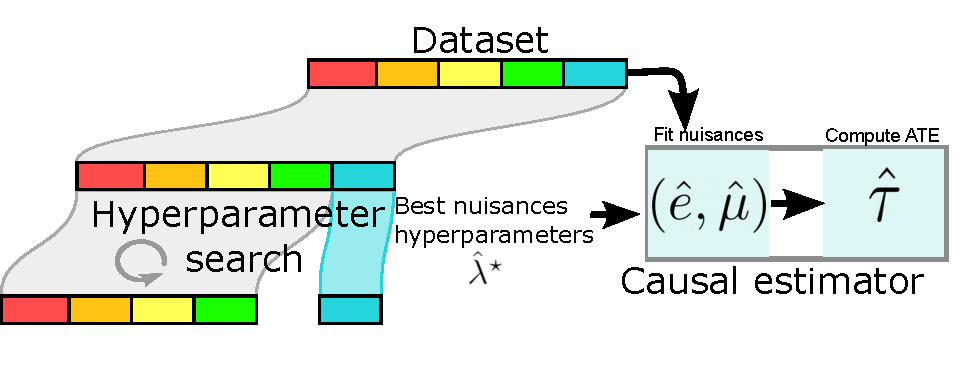
\includegraphics[width=\linewidth]{img_final/hp_search_procedure.pdf}
  \end{minipage}%
\end{figure}
We followed a two-step procedure to train the nuisance models (eg. ($\hat e,
  \hat \mu$) for the AIPW causal estimator), taking inspiration from the
computationally cheap procedure from
\cite[section~3.3]{bouthillier2021accounting}. First, for each nuisance
model, we fit a random parameter search with 5-fold cross validation and 10
iterations on the full dataset. Each iteration fit a model with a random
combination of parameters in a predefined grid, then evaluate the
performance by cross-validation. The best hyper-parameters $\hat
  \lambda^{\star}$ are selected as the ones reaching the minimal score across
all iterations. Then, we feed this parameters to the causal estimator. The
single robust estimators (matching, IPW and TLearner) refit the
corresponding estimator only once on the full dataset, then estimate the
ATE. The doubly-robust estimators use a cross-fitting procedure (K=5) to fit
the nuisances then estimate the ATE. Figure
\ref{apd:fig:hyper_parameter_search} illustrates the procedure and Table
\ref{apd:table:hyper_parameter_search} details the hyper-parameters grid for
the random search.


\begin{table}[]
  \resizebox{\textwidth}{!}{%
    \begin{tabular}{llll}
    \toprule
    {}             & estimator              & nuisance  & Grid                                                                       \\
    Estimator type &                        &           &                                                                            \\
    \midrule
    Linear         & LogisticRegression     & treatment & \{'C': logspace(-3, 2, 10)\}                                               \\
    Linear         & Ridge                  & outcome   & \{'alpha': logspace(-3, 2, 10)\}                                           \\
    Forest         & RandomForestClassifier & treatment & \{'n\_estimators': ['10', '100', '200'], 'max\_depth': ['3', '10', '50']\} \\
    Forest         & RandomForestRegressor  & outcome   & \{'n\_estimators': ['10', '100', '200'], 'max\_depth': ['3', '10', '50']\} \\
    \bottomrule
\end{tabular}

  }\\
  \caption{Hyper-parameter grid used during random search
    optimization.}\label{apd:table:hyper_parameter_search}
\end{table}
\clearpage

\paragraph*{S7 Appendix.}
\label{apd:computing_resources}
{\bf Computing resources.}

The whole project was run on a laptop running Ubuntu 22.04.2 LTS with the following hardware:
CPU 12th Gen Intel(R) Core(TM) i7-1270P with 16 threads and 15 GB of RAM.
\clearpage

\paragraph*{S5 Fig.}
\label{apd:selection_flowchart}
{\bf Selection flowchart.}

\begin{figure}[!htb]
  \centering
  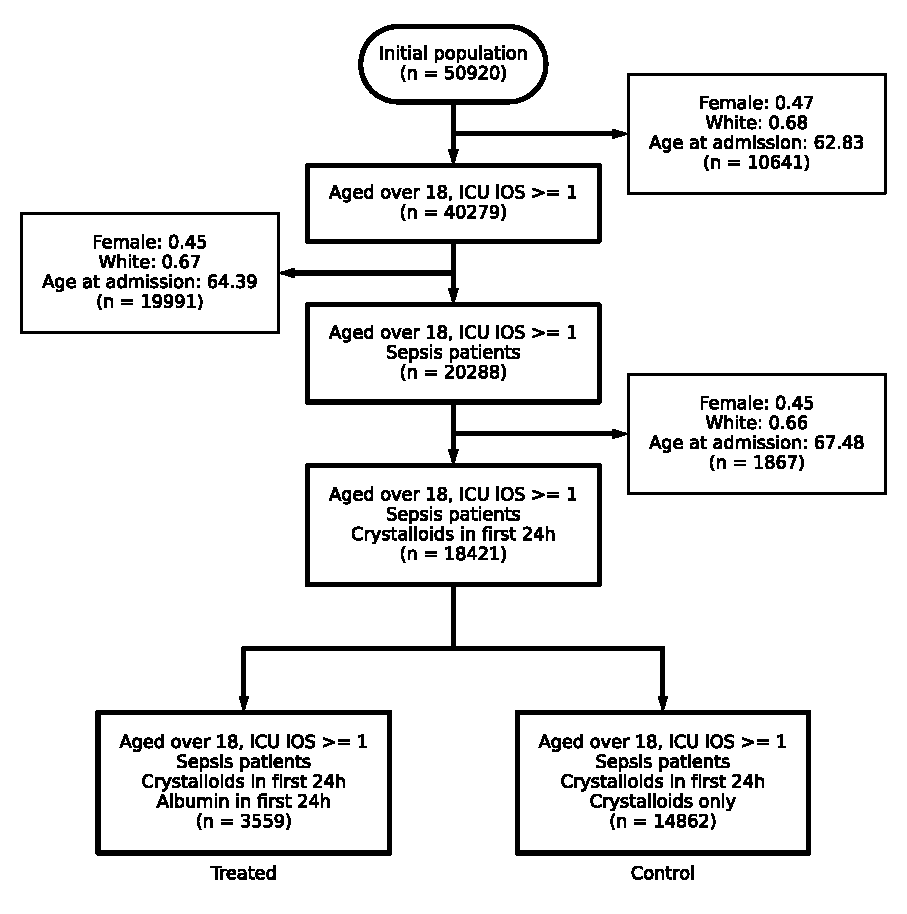
\includegraphics[width=0.7\linewidth]{img_final/albumin_for_sepsis__obs_1d__flowchart_albumin_for_sepsis.pdf}
  \caption{Selection flowchart on MIMIC-IV for the emulated trial.}\label{fig:selection_flowchart}
\end{figure}
\clearpage


\paragraph*{S1 Table.}
\label{apd:albumin_for_sepsis:table1_complete}
{\bf Complete description of the confounders for the main analysis.}
\begin{table}[h!]
  \resizebox{\textwidth}{!}{%
    \begin{tabular}{llllll}
\toprule
{} & Missing &        Overall & Cristalloids only & Cristalloids + Albumin & P-Value \\
                                                  &         &                &                   &                        &         \\
\midrule
n                                                 &         &          18421 &             14862 &                   3559 &         \\
Glycopeptide, n (\%)                               &         &    9492 (51.5) &       7650 (51.5) &            1842 (51.8) &         \\
Beta-lactams, n (\%)                               &         &    5761 (31.3) &       5271 (35.5) &             490 (13.8) &         \\
Carbapenems, n (\%)                                &         &      727 (3.9) &         636 (4.3) &               91 (2.6) &         \\
Aminoglycosides, n (\%)                            &         &      314 (1.7) &         290 (2.0) &               24 (0.7) &         \\
suspected\_infection\_blood, n (\%)                  &         &      170 (0.9) &         149 (1.0) &               21 (0.6) &         \\
RRT, n (\%)                                        &         &      229 (1.2) &         205 (1.4) &               24 (0.7) &         \\
ventilation, n (\%)                                &         &   16376 (88.9) &      12931 (87.0) &            3445 (96.8) &         \\
vasopressors, n (\%)                               &         &    9058 (49.2) &       6204 (41.7) &            2854 (80.2) &         \\
Female, n (\%)                                     &         &    7653 (41.5) &       6322 (42.5) &            1331 (37.4) &         \\
White, n (\%)                                      &         &   12366 (67.1) &       9808 (66.0) &            2558 (71.9) &         \\
Emergency admission, n (\%)                        &         &    9605 (52.1) &       8512 (57.3) &            1093 (30.7) &         \\
Insurance, Medicare, n (\%)                        &         &    9727 (52.8) &       7958 (53.5) &            1769 (49.7) &         \\
myocardial\_infarct, n (\%)                         &         &    3135 (17.0) &       2492 (16.8) &             643 (18.1) &         \\
malignant\_cancer, n (\%)                           &         &    2465 (13.4) &       2128 (14.3) &              337 (9.5) &         \\
diabetes\_with\_cc, n (\%)                           &         &     1633 (8.9) &        1362 (9.2) &              271 (7.6) &         \\
diabetes\_without\_cc, n (\%)                        &         &    4369 (23.7) &       3532 (23.8) &             837 (23.5) &         \\
metastatic\_solid\_tumor, n (\%)                     &         &     1127 (6.1) &        1016 (6.8) &              111 (3.1) &         \\
severe\_liver\_disease, n (\%)                       &         &     1289 (7.0) &         880 (5.9) &             409 (11.5) &         \\
renal\_disease, n (\%)                              &         &    3765 (20.4) &       3159 (21.3) &             606 (17.0) &         \\
aki\_stage\_0.0, n (\%)                              &         &    7368 (40.0) &       6284 (42.3) &            1084 (30.5) &         \\
aki\_stage\_1.0, n (\%)                              &         &    4019 (21.8) &       3222 (21.7) &             797 (22.4) &         \\
aki\_stage\_2.0, n (\%)                              &         &    6087 (33.0) &       4605 (31.0) &            1482 (41.6) &         \\
aki\_stage\_3.0, n (\%)                              &         &      947 (5.1) &         751 (5.1) &              196 (5.5) &         \\
SOFA, mean (SD)                                   &       0 &      6.0 (3.5) &         5.7 (3.4) &              6.9 (3.6) &  <0.001 \\
SAPSII, mean (SD)                                 &       0 &    40.3 (14.1) &       39.8 (14.1) &            42.8 (13.6) &  <0.001 \\
Weight, mean (SD)                                 &      97 &    83.3 (23.7) &       82.5 (24.2) &            86.4 (21.2) &  <0.001 \\
temperature, mean (SD)                            &     966 &     36.9 (0.6) &        36.9 (0.6) &             36.8 (0.6) &  <0.001 \\
mbp, mean (SD)                                    &       0 &    75.6 (10.2) &       76.3 (10.7) &             72.4 (7.2) &  <0.001 \\
resp\_rate, mean (SD)                              &       9 &     19.3 (4.3) &        19.6 (4.4) &             18.0 (3.8) &  <0.001 \\
heart\_rate, mean (SD)                             &       0 &    86.2 (16.3) &       86.2 (16.8) &            86.5 (14.3) &   0.197 \\
spo2, mean (SD)                                   &       4 &     97.4 (2.2) &        97.3 (2.3) &             98.0 (2.1) &  <0.001 \\
lactate, mean (SD)                                &    4616 &      3.0 (2.5) &         2.8 (2.4) &              3.7 (2.6) &  <0.001 \\
urineoutput, mean (SD)                            &     301 &    24.0 (52.7) &       24.7 (58.2) &            21.1 (16.6) &  <0.001 \\
admission\_age, mean (SD)                          &       0 &    66.3 (16.2) &       66.1 (16.8) &            67.3 (13.1) &  <0.001 \\
delta mortality to inclusion, mean (SD)           &   11121 &  316.9 (640.2) &     309.6 (628.8) &          365.0 (708.9) &   0.022 \\
delta intervention to inclusion, mean (SD)        &   14862 &      0.3 (0.2) &         nan (nan) &              0.3 (0.2) &     nan \\
delta inclusion to intime, mean (SD)              &       0 &      0.1 (0.2) &         0.1 (0.2) &              0.1 (0.1) &   0.041 \\
delta ICU intime to hospital admission, mean (SD) &       0 &      1.1 (3.7) &         1.0 (3.7) &              1.6 (3.4) &  <0.001 \\
los\_hospital, mean (SD)                           &       0 &    12.6 (12.5) &       12.6 (12.5) &            12.9 (12.4) &   0.189 \\
los\_icu, mean (SD)                                &       0 &      5.5 (6.7) &         5.5 (6.5) &              5.5 (7.2) &   0.605 \\
\bottomrule
\end{tabular}

  }\\
  \caption{Characteristics of the trial population measured on the first 24
    hours of ICU stay. \\
    Risk scores (AKI, SOFA, SAPSII) and lactates have been summarized as the
    maximum value during the 24 hour period for each stay. Total cumulative urine output has
    been computed. Other variables have been aggregated by taking mean during
    the 24 hour period.}\label{apd:table:albumin_for_sepsis:table1_complete}
\end{table}
\clearpage

\paragraph*{S6 Fig.}
\label{apd:causal_diagram_albumin}
{\bf Directed Acyclic Graph.}

The expert DAG in figure depicts the known causal links between these
variables.

\begin{figure}[h!]
  \centering%
  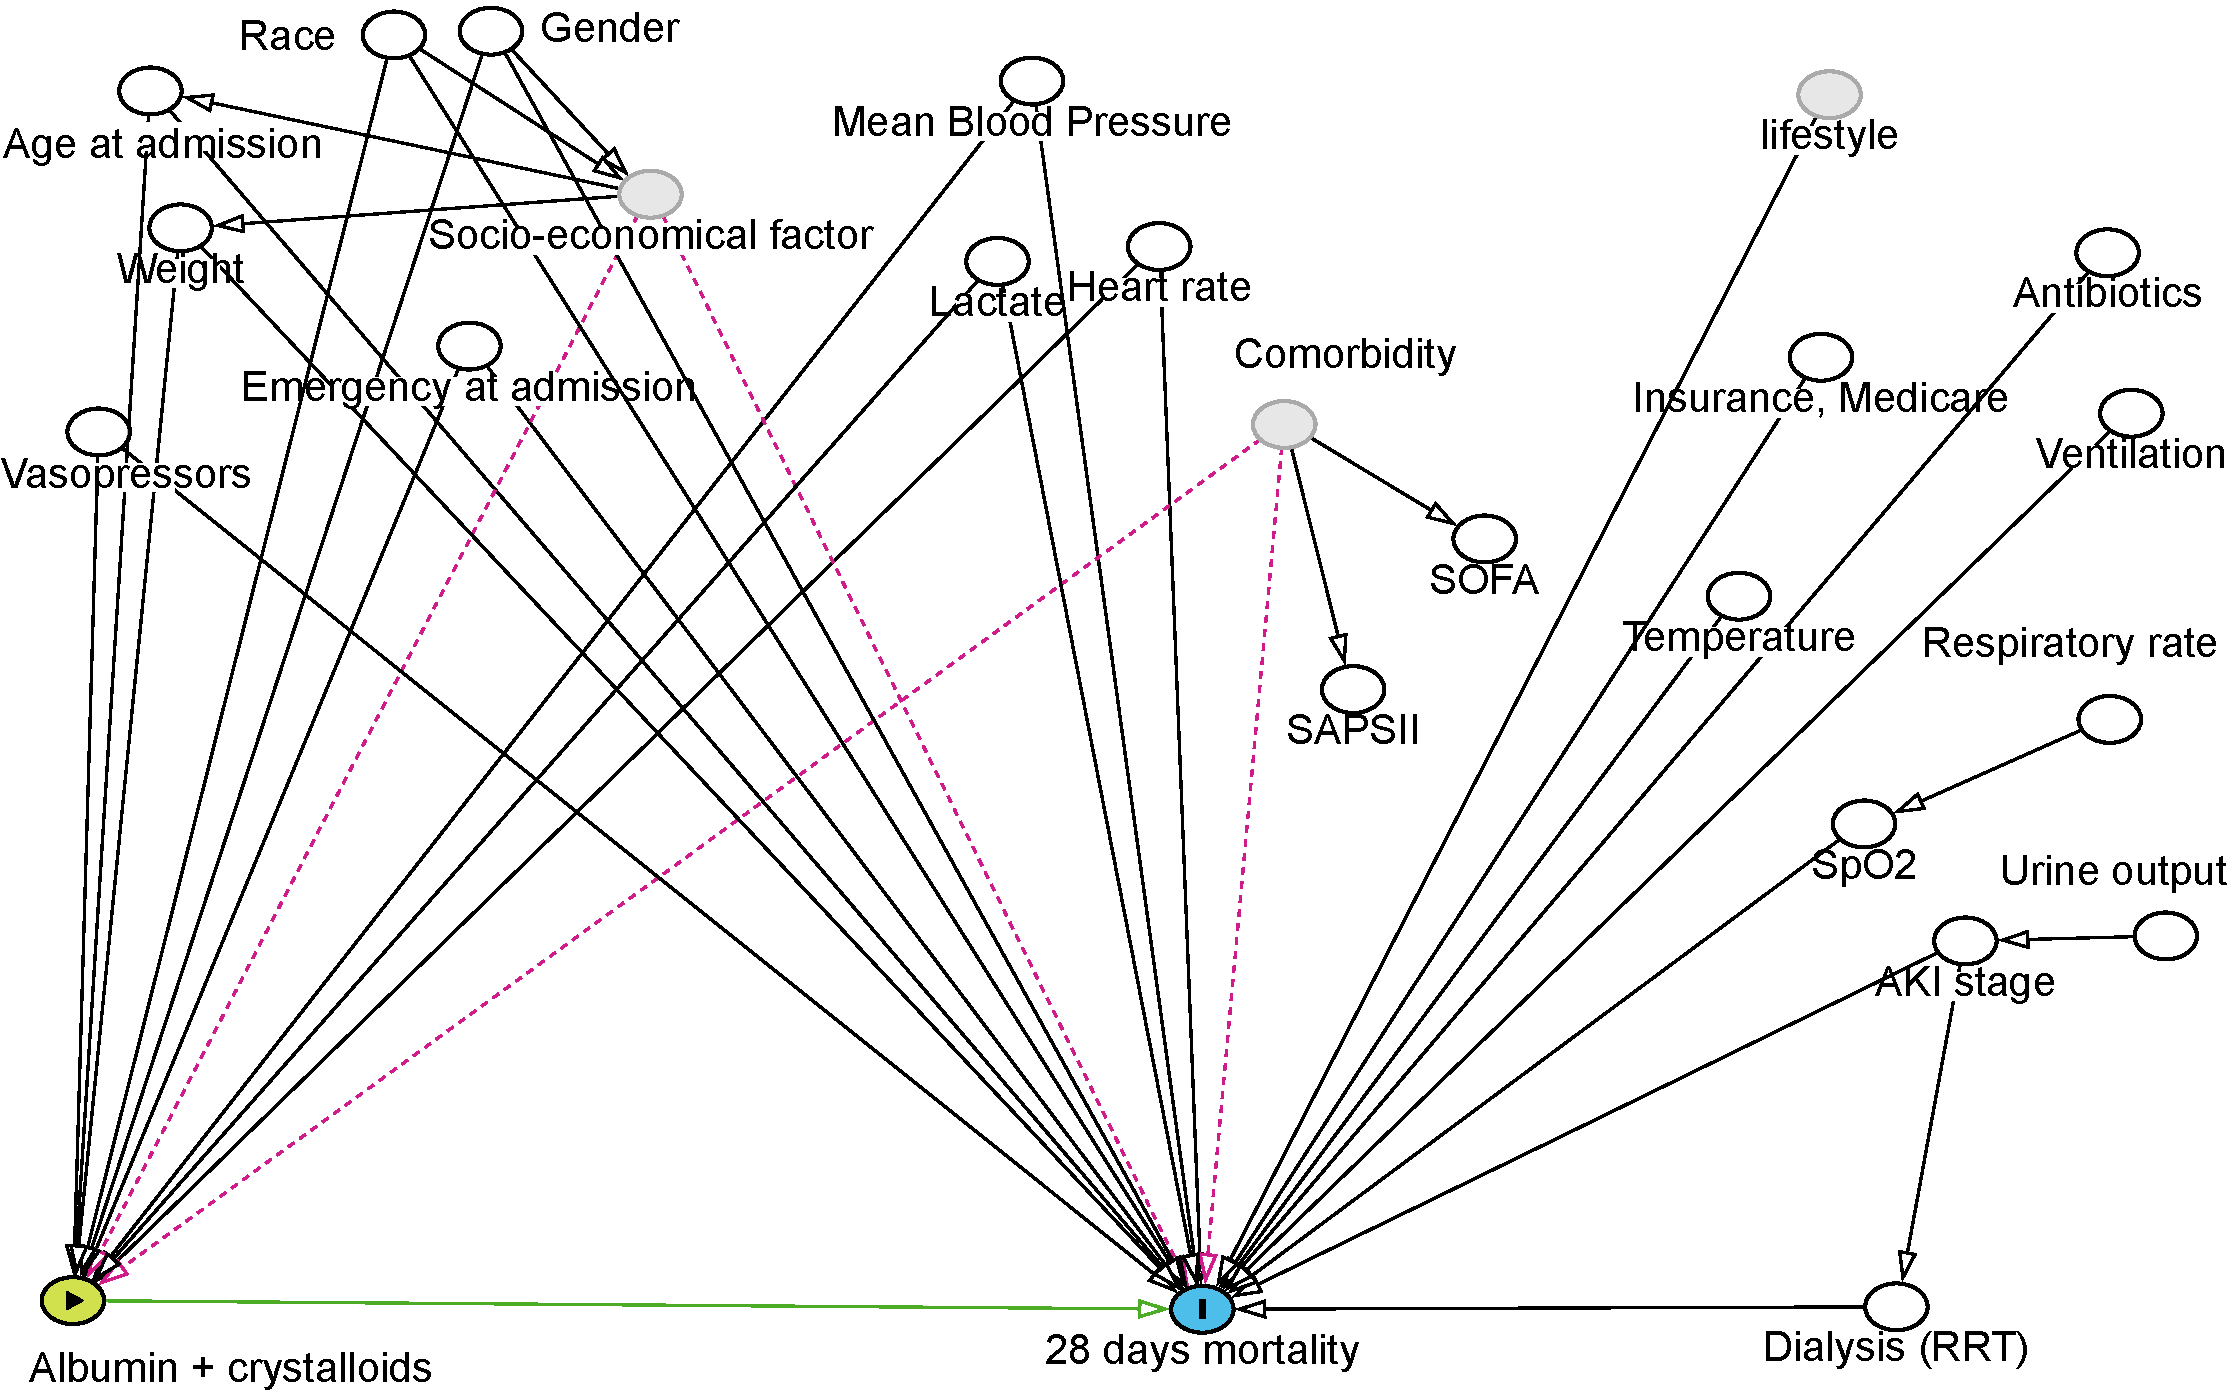
\includegraphics[width=\linewidth]{img_final/dagitty_graph.pdf}
  \caption{\textbf{Causal graph for the Albumin vs crystalloids emulated
      trial} -- The
    green arrow indicates the effect studied. Black arrows show causal links
    known to medical expertise. Dotted red arrows highlight confounders not directly
    observed. For readability, we draw only the most important edges from an
    expert point of view. All white nodes correspond to variables included in
    our study.}\label{fig:causal_diagram_albumin}
\end{figure}
\clearpage


\paragraph*{S7 Fig.}
\label{apd:detailed_results}
{\bf Complete results for the main analysis.}

Compared to Figure \ref{fig:vibration_analysis}, we also report in
Figure \ref{apd:fig:detailed_results} the estimates for Causal forest
estimators and other choices of feature aggregation (first and last).
\begin{figure}[h!]
  \centering
  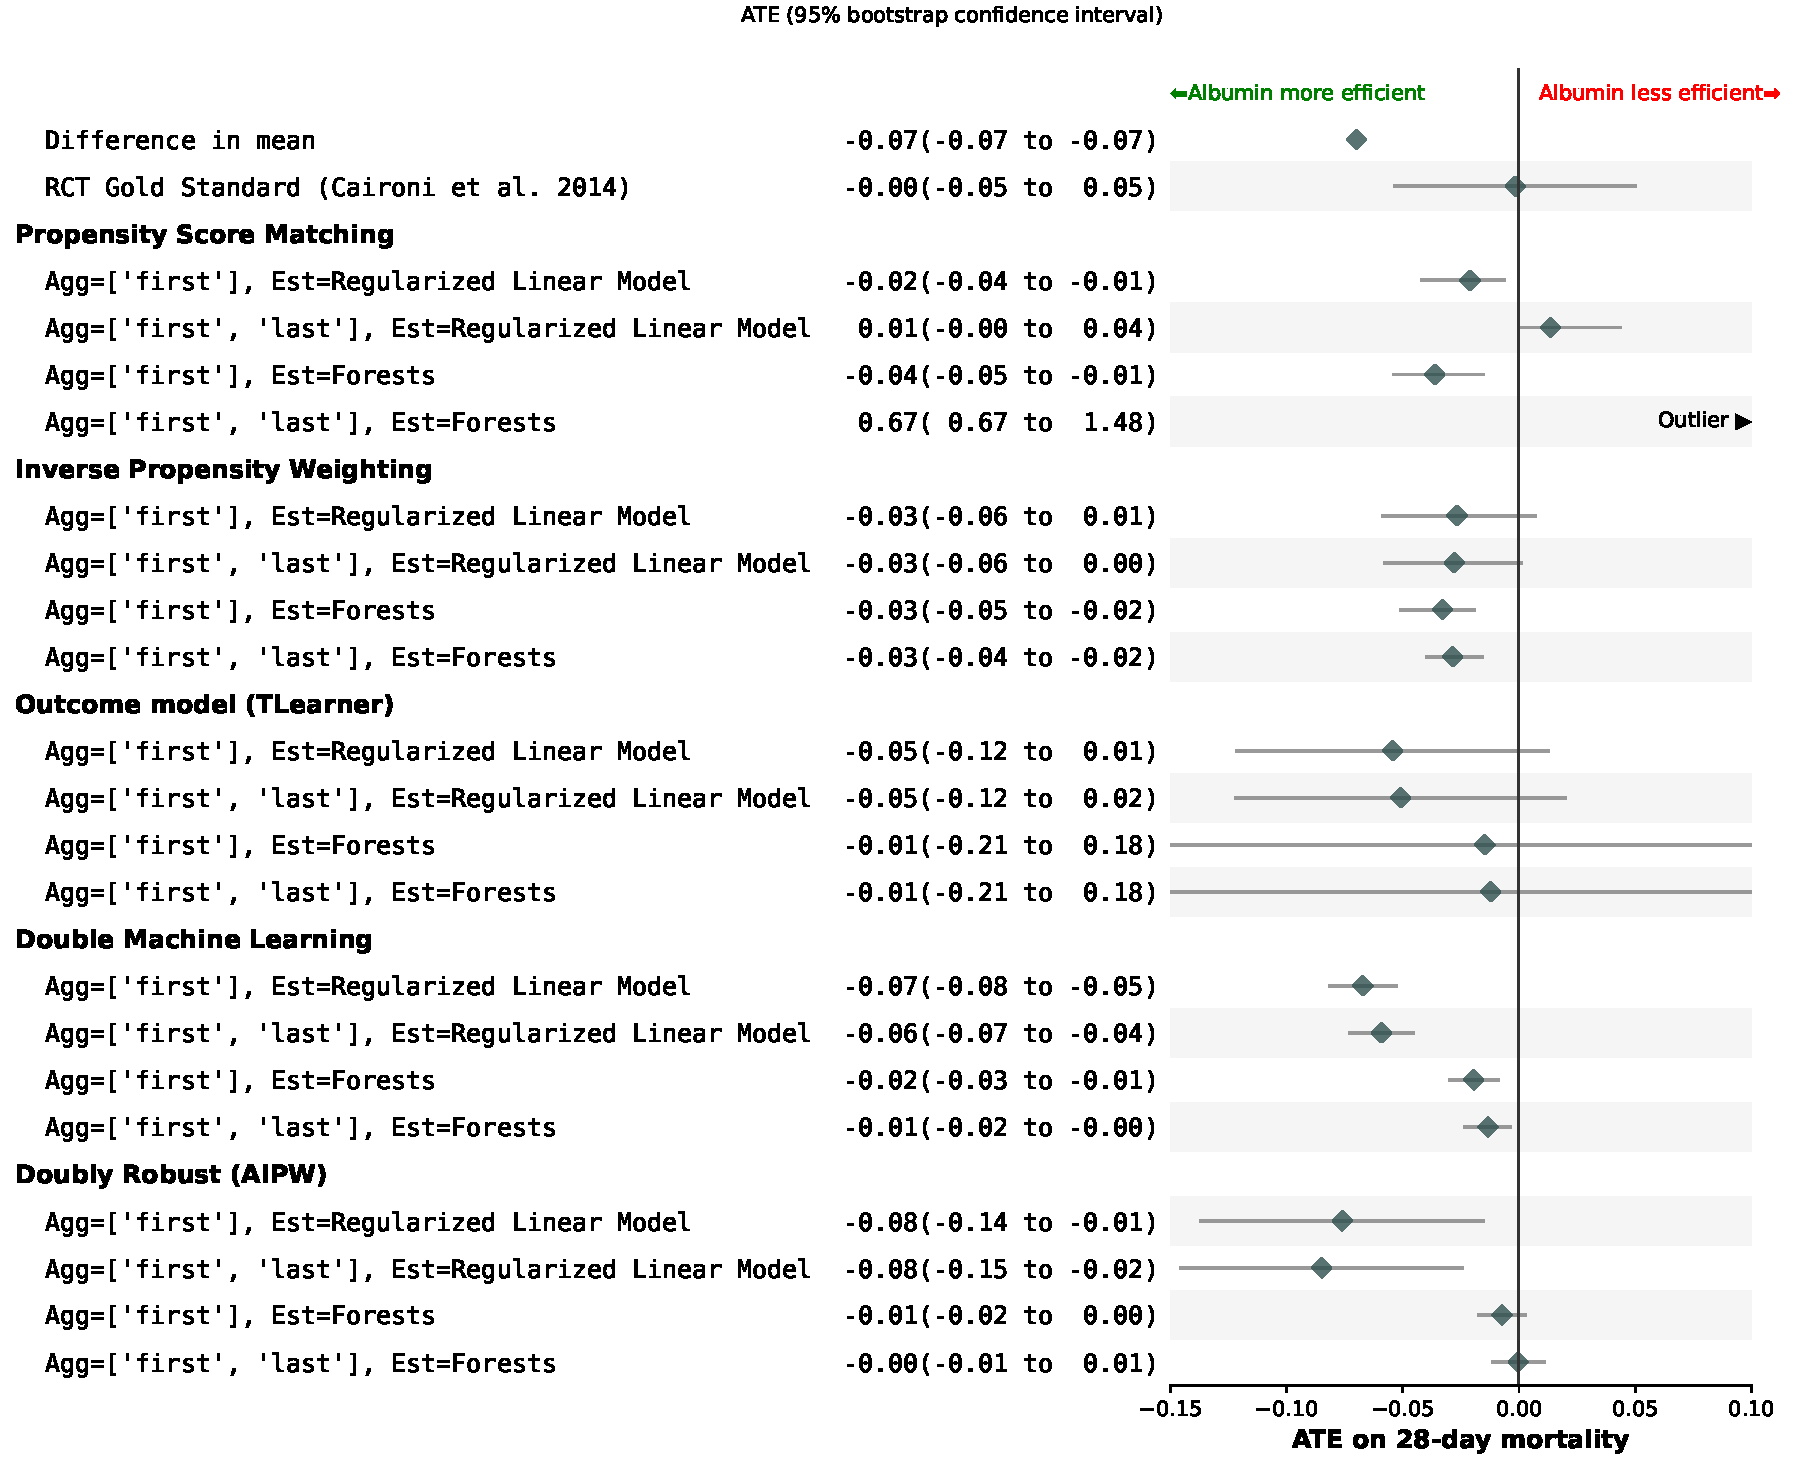
\includegraphics[width=\linewidth]{img_final/main_vibration_analysis_supp.pdf}
  \caption{Full sensitivity analysis: The estimators with forest nuisances
    point to no effect for almost every causal estimator consistently with the
    RCT gold standard. Only matching with forest yields an unconvincingly high
    estimate. Linear nuisance used with doubly robust methods suggest a
    reduced mortality risk for albumin. The choices of aggregation only
    marginally modify the results expect for propensity score matching. The
    green diamonds depict the mean effect and the bar are the 95\% confidence
    intervals obtained by 50 bootstrap
    repetitions.}\label{apd:fig:detailed_results}
\end{figure}
\clearpage

\paragraph*{S8 Fig.}
\label{apd:detailed_results_itb}
{\bf Complete results for the Immortal time bias.}
\clearpage


Compared to Figure \ref{fig:vibration:itb}, we also report in Figure
\ref{apd:fig:detailed_results_itb} the estimates for Double Machine Learning,
Inverse Propensity Weighting for both Random Forest and Ridge Regression.
Feature aggregation was concatenation of first and last for all estimates.

\begin{figure}[h!]
  \centering
  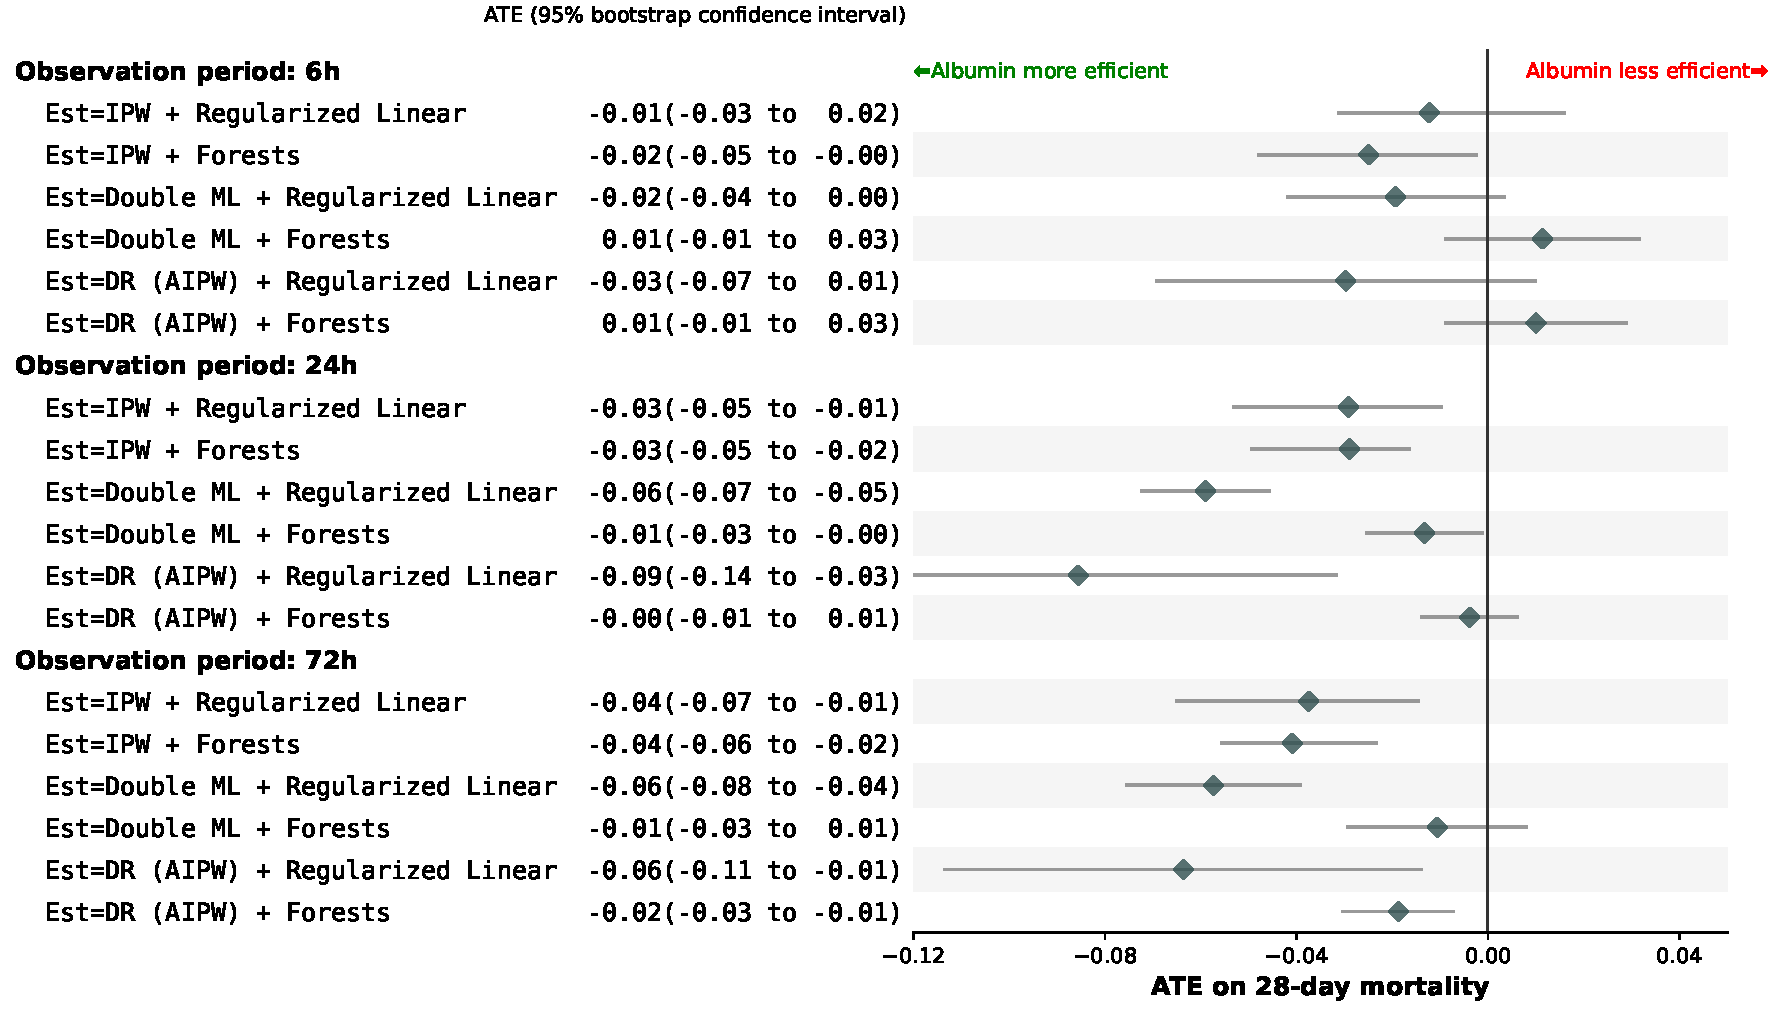
\includegraphics[width=\linewidth]{img_final/itb__dr_forest_agg_first_last__bs_30_supp.pdf}
  \caption{Sensitivity analysis for immortal time bias: Every choice of
    estimates show an improvement of the albumin treatment when increasing the
    observation period, thus increasing the blank period between inclusion and
    administration of albumin. Aggregation was concatenation of first and last
    features. The green diamonds depict the mean effect and the bar are the
    95\% confidence intervals obtained by 50 bootstrap
    repetitions.}\label{apd:fig:detailed_results_itb}
\end{figure}
\clearpage

\paragraph*{S8 Appendix.}
\label{apd:vibration_analysis_for_confounders}
{\bf Deviating from expert ignorability -- Impact of smaller confounders sets.}


We conducted a dedicated vibration analysis on the different choices of
confounders. We created three confounder subsets in addition to all
confounders (24 variables): all confounders without antibiotics
(Glycopeptides, Beta-lactams, Carbapenems, Aminoglycosides), all confounders
without any measurement (weight, lactate, heart rate,
spo2, mbp, urine output, temperature, AKI stage, SAPSII, respiratory rate, SOFA), only
socio-demographics (admission age, female, emergency admission,
insurance--medicare, race).

Figure \ref{fig:vibration:confounders} shows that small
deviation from the ignorability assumptions is tolerable: for example, removing
antibiotics does not impact the estimate. However, the larger the
deviation from graph \ref{fig:causal_diagram_albumin}, the larger the bias
compared to the gold-standard. Adjusting only for socio-demographics features
is the closest from an unadjusted risk difference, indicating that we lack
important confounders on the patient health state. This stability of the
treatment effect estimator once sufficient confounders have been included has
already been described and suggested as a confounder selection method
\cite{loh2021confounder}.
\clearpage

\paragraph*{S9 Fig.}
\label{apd:vibration_analysis_for_aggregation}
{\bf Vibration analysis for aggregation.}

We conducted a dedicated vibration analysis on the different choices of
features aggregation, studying the impact on the estimated ATE. We also
studied if some choices of aggregation led to substantially poorer overlap.

We assessed overlap with two different methods. As recommended by
\cite{austin2015moving}, we did a graphical assessment by plotting the
distribution of the estimated. The treatment model hyper-parameters were chosen
by random search, then predicted propensity scores were obtained by refitting
this estimator with cross-fitting on the full dataset.

As shown in Figure \ref{apd:fig:albumin_for_sepsis:overlap_measure}, we did not find substantial differences between methods
when plotting graphically the distribution of the estimated propensity score.

\begin{figure}[h!]
  \centering
  \begin{subfigure}[b]{0.45\linewidth}
    \centering
    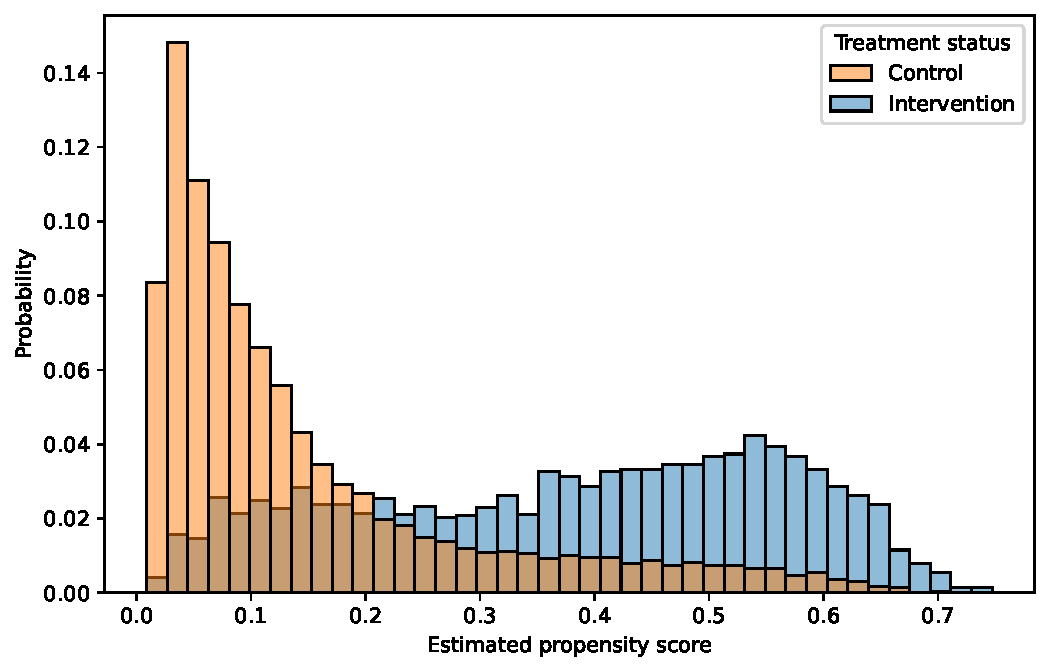
\includegraphics[width=\linewidth]{img_final/sensitivity__ps_distribution__first_last_median__Forests.pdf}
    \caption{}\label{apd:fig:albumin_for_sepsis:overlap_measure_first_last_median}
  \end{subfigure}
  \hfill
  \begin{subfigure}[b]{0.45\linewidth}
    \centering
    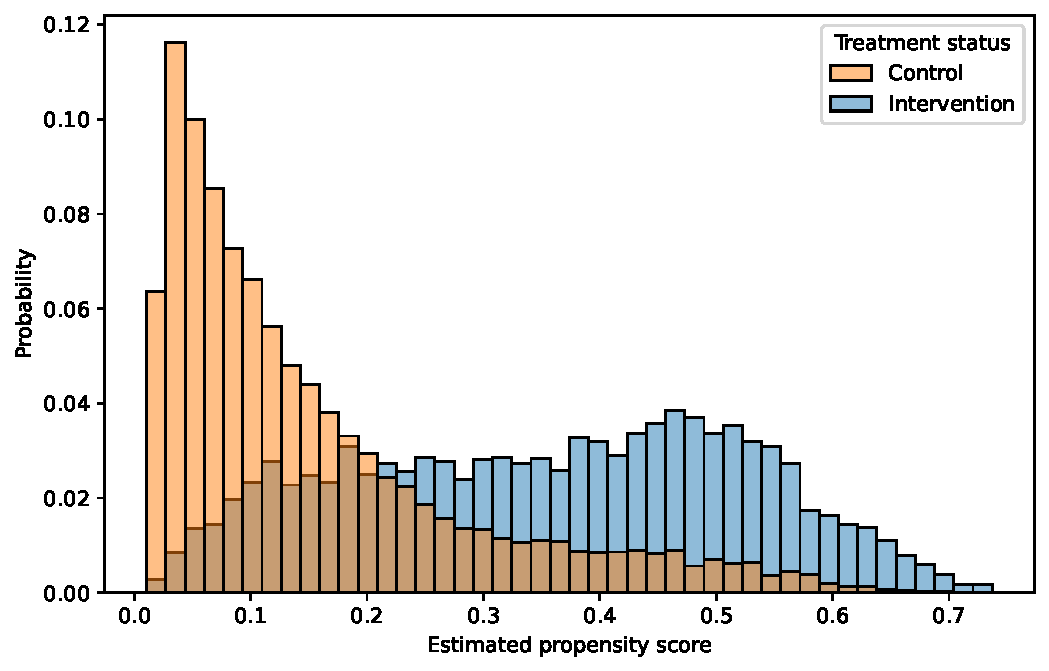
\includegraphics[width=\linewidth]{img_final/sensitivity__ps_distribution__first__Forests.pdf}
    \caption{}\label{apd:fig:albumin_for_sepsis:overlap_measure_first}
  \end{subfigure}
  \caption{Different choices of aggregation yield qualitatively close
    distributions of the propensity score: Figure
    \ref{apd:fig:albumin_for_sepsis:overlap_measure_first_last_median})a)
    shows a concatenation of first, last and median measures whereas Figure
    \ref{apd:fig:albumin_for_sepsis:overlap_measure_first})b) shows an
    aggregation by taking the first measure only. The underlying treatment
    effect estimator is a random forest. }\label{apd:fig:albumin_for_sepsis:overlap_measure}
\end{figure}

We also used normalized total variation (NTV) as a summary statistic of the
estimated propensity score to measure the distance between treated and control
population \cite{doutreligne2023select}. This statistic varies between 0 --
perfect overlap -- and 1 -- no overlap at all. Fig
\ref{apd:fig:albumin_for_sepsis:vibration_analysis_for_aggregation} shows no
marked differences in overlap as measured by NTV between aggregation choices,
comforting us in our expert-driven choice of the aggregation: a concatenation
of first and last feature observed before inclusion time.

\begin{figure}[h!]
  \centering
  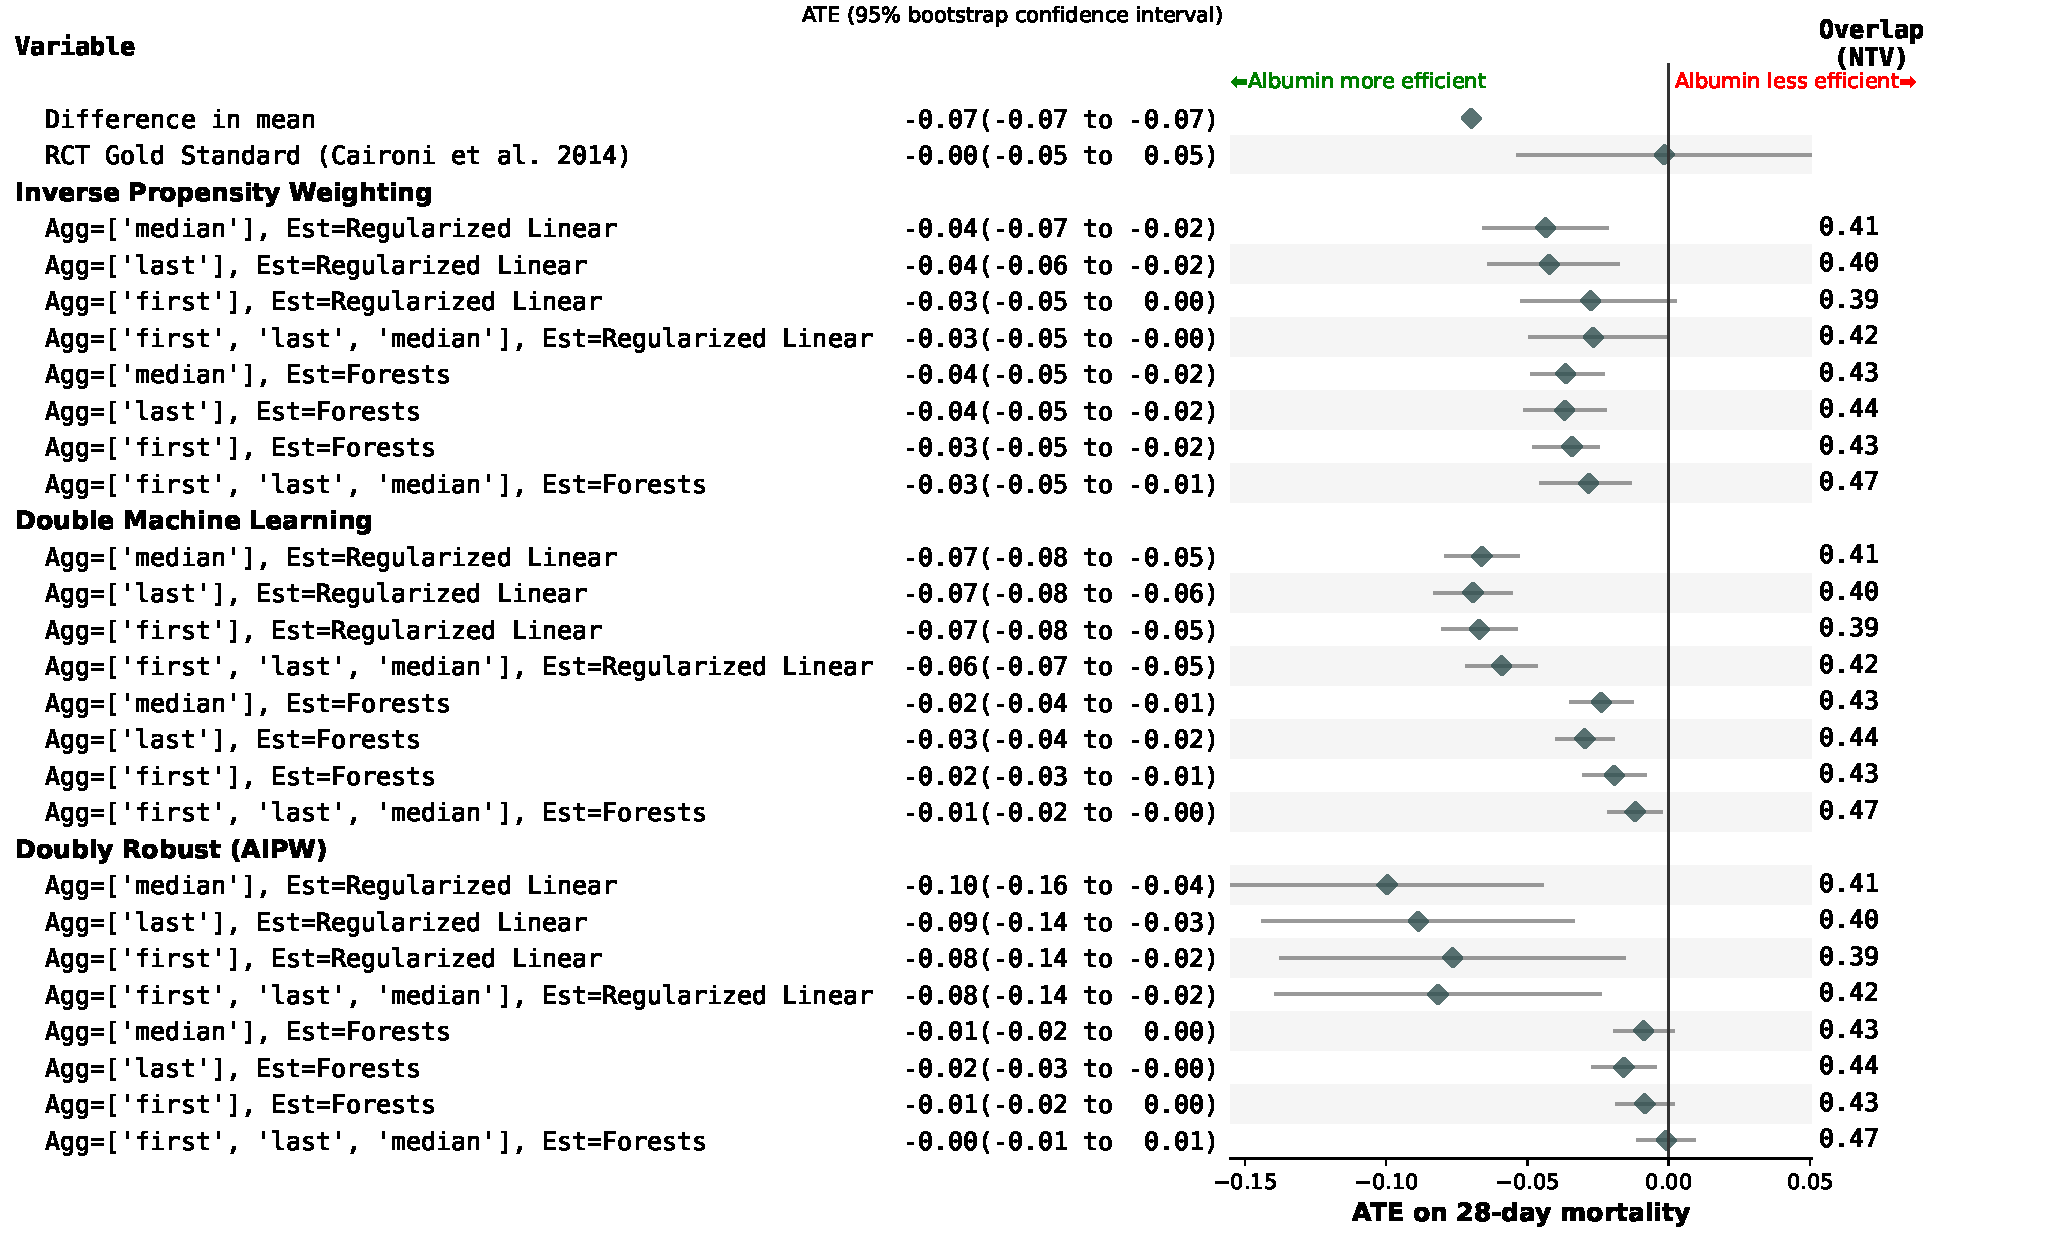
\includegraphics[width=1.0\linewidth]{img_final/sensitivity_feature_aggregation_albumin_for_sepsis__bs_50.pdf}
  \caption{Vibration analysis dedicated to the aggregation choices. The
    choices of aggregation only marginally modify the results. When assessed
    with Normalized Total Variation, the overlap assumption is respected for all
    our choices of aggregation. The green diamonds depict the mean effect and
    the bar are the 95\% confidence intervals obtained by 50 bootstrap
    repetitions.}\label{apd:fig:albumin_for_sepsis:vibration_analysis_for_aggregation}
\end{figure}
\clearpage


\paragraph*{S8 Appendix.}
\label{apd:hte}
{\bf Details on treatment heterogeneity analysis.}
\textbf{Detailed estimation procedure}

The estimation of heterogeneous effect based on Double Machine Learning adds
another step after the computation, regressing the residuals of the outcome
nuisance $\tilde{Y} - \mu(X)$ against the residuals of the treatment nuisance
$\tilde{A} = A - e(X)$ with the heterogeneity features $X_{CATE}$. Noting the
final CATE model $\theta$, Double ML solves:

$$\argmin_{\theta} \mathbb E_n \big[(\tilde{Y} - \tau (X_CATE) \cdot \tilde{A})^2\big ]$$

Where $\tilde{Y} = Y - \hat m(X)$ and $\tilde{A} = A - \hat e(X)$

To avoid the over-fitting of this last regression model, we split the dataset of
the main analysis into a train set (size=0.8) where the causal estimator and the final
model are learned, and a test set (size=0.2) on which we report the predicted Conditional Average
Treatment Effects.

\textbf{Known heterogeneity of treatment for the emulated trial}\label{apd:cate_literature}

\cite{caironi2014albumin} observed statistical differences in the post-hoc
subgroup analysis between patient with and without septic shock at inclusion.
They found increasing treatment effect measured as relative risk for patients
with septic shock (RR=0.87; 95\% CI, 0.77 to 0.99 vs 1.13;95\% CI, 0.92 to 1.39).

\cite{safe2007saline} conducted a post-hoc subgroup analysis of patients with or
without brain injury --defined as Glasgow Coma Scale between 3 to 8--. The
initial population was patients with traumatic brain injury (defined as history
or evidence on A CT scan of head trauma, and a GCS score <= 13). They found
higher mortality rate at 24 months in the albumin group for patients with severe
head injuries.

\cite{zhou2021early} conducted a subgroup analysis on age (<60 vs >60), septic
shock and sex. They conclude for increasing treatment effect measured as
Restricted Mean Survival Time for Sepsis vs septic shock (3.47 vs. 2.58), for
age >=60 (3.75 vs 2.44), for Male (3.4 vs 2.69). None of these differences were
statistically significant.

\textbf{Vibration analysis}\label{apd:cate_results}

The choice of the final model for the CATE estimation should also be informed
by statistical and clinical rationals. Figure
\ref{apd:fig:albumin_for_sepsis:cate_boxplot_forest} shows the distribution of
the individual effects of a final random forest estimator, yielding CATE
estimates that are not consistent with the main ATE analysis. Figure
\ref{apd:fig:albumin_for_sepsis:cate_age_forest_failure} shows that the choice
of this final model imposes an inductive bias on the form of the heterogeneity
and different sources of noise depending of the nature of the model. A random
forest is noisier than a linear model. Figure
\ref{apd:fig:albumin_for_sepsis:cate_age_forest_failure} shows the difference
of modelization on the subpopulation of non-white male patients without septic
shock. One can see that the decreasing linear trend is reflected by the
random forest model only for patients aged between 55 and 80.

\begin{figure}[h!]
  \centering
  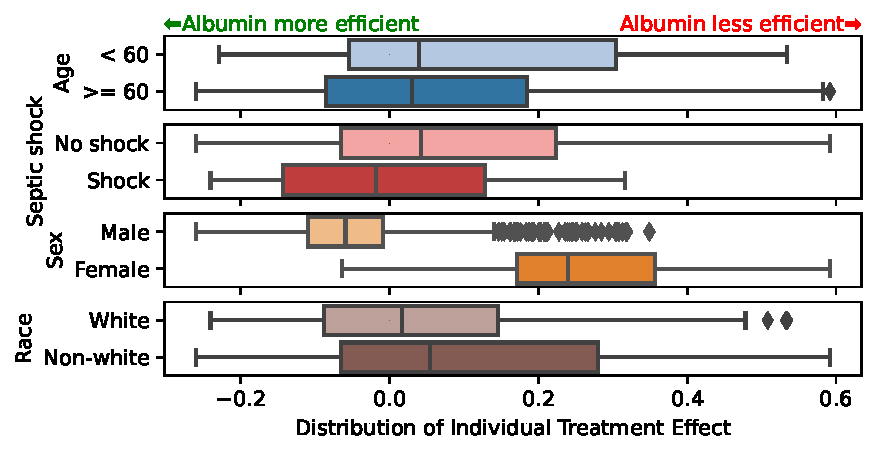
\includegraphics[width=0.8\linewidth]{img_final/boxplot_est__DML__nuisances__Forests__final_RF.pdf}
  \caption{Distribution of Conditional Average Treatment effects on sex, age,
    race and pre-treatment septic shock estimated with a final forest
    estimator. The CATE are positive for each subgroups, which is not
    consistent with the null treatment effect obtained in the main analysis.
    The boxes contain between the 25th and 75th percentiles of the CATE
    distributions with the median indicated by a vertical line. The whiskers
    extends to 1.5 the inter-quartile range of the
    distribution.}\label{apd:fig:albumin_for_sepsis:cate_boxplot_forest}
\end{figure}

\begin{figure}
  \centering
  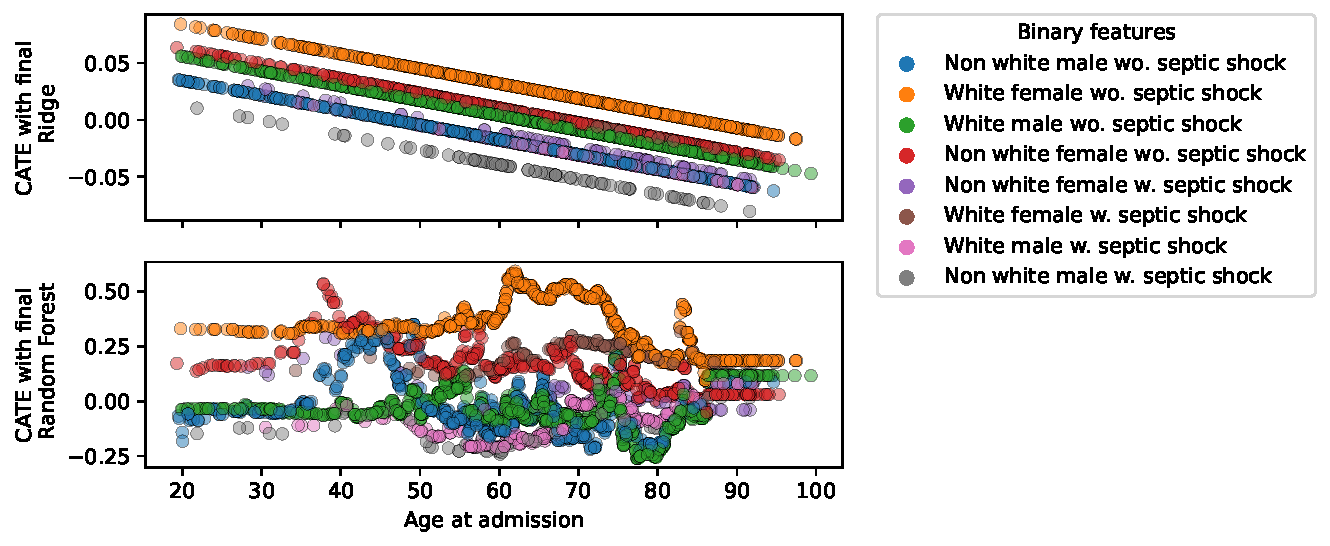
\includegraphics[width=\linewidth]{img_final/cate_all_category_random_forest.pdf}
  \caption{Distribution of Conditional Average Treatment effects on sex, age,
    race and pre-treatment septic shock plotted for different ages. On the top
    the final estimator is a linear model; on the bottom, it is a random
    forest. The forest-based CATE displays more noisy trends than the
    linear-based CATE. This suggest that the flexibility of the random forest
    might be underfitting the data.}\label{apd:fig:albumin_for_sepsis:cate_age_forest_failure}
\end{figure}

\begin{figure}
  \centering
  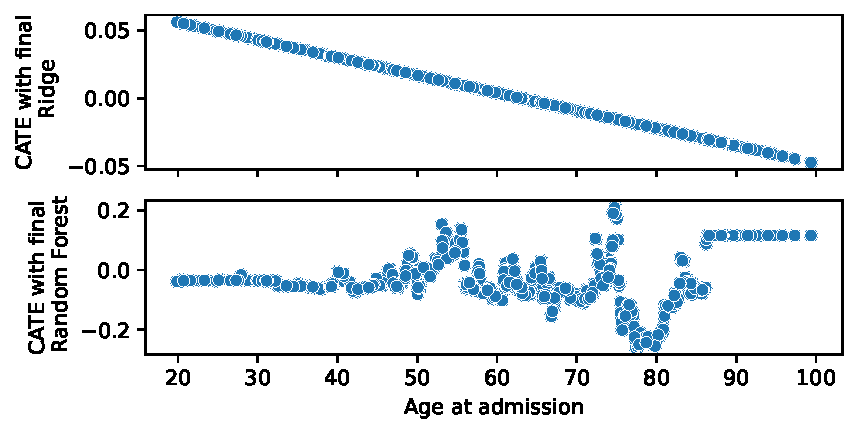
\includegraphics[width=\linewidth]{img_final/cate_shock_random_forest.pdf}
  \caption{Figure \ref{apd:fig:albumin_for_sepsis:cate_age_forest_failure} on
    the subpopulation of white male patients without septic shock. Contrary to
    the ridge regression (on top) inducing a nicely interpretable trend, using
    random forests as the final estimator failed to recover CATE on ages: the
    predicted estimates do not exhibit any trend and display inconsistently
    large effect sizes, suggesting data underfitting.
  }\label{apd:fig:albumin_for_sepsis:cate_failure}
\end{figure}
\clearpage

\paragraph*{S9 Appendix.}
\label{apd:risk_assessment_scores}
{\bf Risk assessment tools for prevention.}


\textbf{An example of nationally deployed cardiovascular prevention tool: QRISK}

The QRISK is a risk score widely used in the UK to assess 10-year
cardio-vascular risk \cite{hippisley2017development}. It is well calibrated
and have satisfactory discriminative performances. As such, it is recommended
by the national regulatory agency to engage the patient into various
preventive interventions such as physical activity, cardio-protective diet,
statins initiation \cite{guideline2023cardiovascular}. The NICE argues in favor
of systematic screening of cardio-vascular risks to increase the number of
people receiving statins \cite{guideline2023cardiovascular}.

The QRISK seems to mostly inform the initiation of statins for patients
exceeding 10\% 10-year CVD risk (as measured with QRISK) following the 2014
NICE guidelines \cite{rabar2014lipid}.

They base their evidence on a cost-effectiveness analysis choosing the 10\%
threshold to optimize quality-adjusted life year at the population level based
on the cost of life-long statin treatments \cite{guthrie2023competing}. This
study assumes constant statins effect among different CVD risk groups:
\emph{It is assumed that the risk ratios given for treatment with each class
  of statins are constant regardless of the baseline CV risk --that is, someone
  with low CV risk will receive the same proportional reduction in that risk as
  would someone with a high CV risk. This is unproven, but is consistent with
  the results of meta-analysis carried out by the Cholesterol Treatment
  Trialists, which found effectiveness to be broadly similar for those at
  different risk levels.} This hypothesis is supported by the meta-analysis of
at least for the important risk factors of sex and age \cite{brugts2009benefits}. It is also assumed that these risk ratios are constant regardless of
baseline LDL-cholesterol levels. More recent work showed that risk ratio
stratified by patient baseline CVD risk levels were not significant, raising
doubts about the overall efficacy of statins for primary prevention \cite{byrne2019statins}.

The updated guidelines from the US Preventive Services Task Force found
respectively moderate and small net benefice of statins for patients aged 40
to 75 with above 10\% CVD risk and from 7.5 to 10\% without history of CVD
\cite{chou2022statin}. They conclude that the evidence is insufficient to
determine the balance of benefits and harms of statin use for the primary
prevention of CVD events and mortality in adults 76 years or older with no
history of CVD.


\textbf{Critics on the efficiency of systematic screening points to treatment heterogeneity}

On the other side, the WHO systematic review on systematic screening for
cardio-vascular risks from 2019 \cite{eriksen2021effectiveness} is
categorical on the poor effectiveness of systematic cardiovascular risk
screening, consistently with the Cochrane review on poor effectiveness
\cite{krogsboll2012general}. For the WHO, systematic screening leads to
over-diagnosis and over-treatment. They mention in their argumentation no
positive effect of statins and even adverse effect for mild hypertension
\cite{diao2012pharmacotherapy}. They also mention critics against poor
uptake of the systematic screening in UK or Albany leading to documented
social bias in the screened population: for example, in the UK, treatment
heterogeneity at a given risk level \cite{van2013efficiency} or documentation
of social inequities of health checks \cite{krska2016implementation}.

\begin{itemize}
  \item The first critic shows that the augmentation of statin prescriptions
        (up to 400\% increase for high risk patients), has been associated with
        heterogeneity in statin prescriptions for given risk score levels
        \cite{van2013efficiency}. Low risk patients have been over-prescribed
        and high risk patient under-prescribed, resulting in questionable overall
        improvement. In this case, the constant effect
        hypothesis of statin proposed by the NICE cost-effectiveness study is in doubt.
        Having access to sources of heterogeneity would help to optimize
        treatment allocation. The risk score might capture interesting
        heterogeneity directions, but we lack data from RCTs to draw such conclusions.

  \item  The second critic points to a treatment allocation bias for risk
        assessment. It seems that mostly socially advantaged patients are
        receiving risk assessment and thus the possibility to be treated with
        statins. This critic also points to treatment heterogeneity.
        Suppose that every patient benefits the same from statins, then even a
        small part of the population --such as the socially advantaged at more
        than 10\% risk-- would benefit from it and make the intervention
        effective at the population level.
\end{itemize}



\textbf{NICE evidence for statin efficacy}

In the NICE analysis, three trials weight for more than 70\% of the effect. All
focus on high risk patients and secondary prevention. It is not clear if
those effects are used for the cost-effectiveness.

\begin{itemize}
  \item LIPID \cite{long1998prevention} (32\% of the effect): 9,014 patients with a history of
        myocardial infraction or hospitalization ie. secondary prevention.
  \item PROSPER \cite{shepherd2002pravastatin} (22\% of the effect): an elderly cohort of
        5,804 men and women with, or at high risk of developing, cardiovascular
        disease and stroke.
  \item ALLHAT-LLT \cite{antihypertensive2002major} (23\% of the effect): 10,355 patients age more than 55
        years and stage 1 or 2 hypertension with at least 1 additional CHD risk
        factor.
\end{itemize}
\clearpage



\section*{Acknowledgments}

We thank all the PhysioNet team for their encouragements and support. In
particular: Fredrik Willumsen Haug, João Matos, Luis Nakayama, Sicheng Hao, Alistair Johnson.

\nolinenumbers

% Either type in your references using
% \begin{thebibliography}{}
% \bibitem{}
% Text
% \end{thebibliography}
%
% or
%
% Compile your BiBTeX database using our plos2015.bst
% style file and paste the contents of your .bbl file
% here. See http://journals.plos.org/plosone/s/latex for 
% step-by-step instructions.
% 
%%% TODO: copy the content of .bst once all manuscript is ok
\bibliography{references}
% \begin{thebibliography}{10}

%   \bibitem{bib1}
%   Conant GC, Wolfe KH.
%   \newblock {{T}urning a hobby into a job: how duplicated genes find new
%     functions}.
%   \newblock Nat Rev Genet. 2008 Dec;9(12):938--950.

%   \bibitem{bib2}
%   Ohno S.
%   \newblock Evolution by gene duplication.
%   \newblock London: George Alien \& Unwin Ltd. Berlin, Heidelberg and New York:
%   Springer-Verlag.; 1970.

%   \bibitem{bib3}
%   Magwire MM, Bayer F, Webster CL, Cao C, Jiggins FM.
%   \newblock {{S}uccessive increases in the resistance of {D}rosophila to viral
%     infection through a transposon insertion followed by a {D}uplication}.
%   \newblock PLoS Genet. 2011 Oct;7(10):e1002337.

% \end{thebibliography}



\end{document}

